En este capítulo se recoge el diseño de la arquitectura del sistema informático, el diseño físico de datos y el diseño detallado de la interfaz de usuario.
\section{Diseño del sistema}
\subsection{Arquitectura del sistema}

La arquitectura del sistema se basa en un modelo de flujo de datos enriquecido, donde la información es captada, procesada y transformada mediante técnicas de analítica avanzada antes de su almacenamiento y exposición. El diseño estructural, representado en la Figura \ref{fig:arquitectura}, se divide en las siguientes etapas funcionales:

\begin{figure}[H]
    \centering
    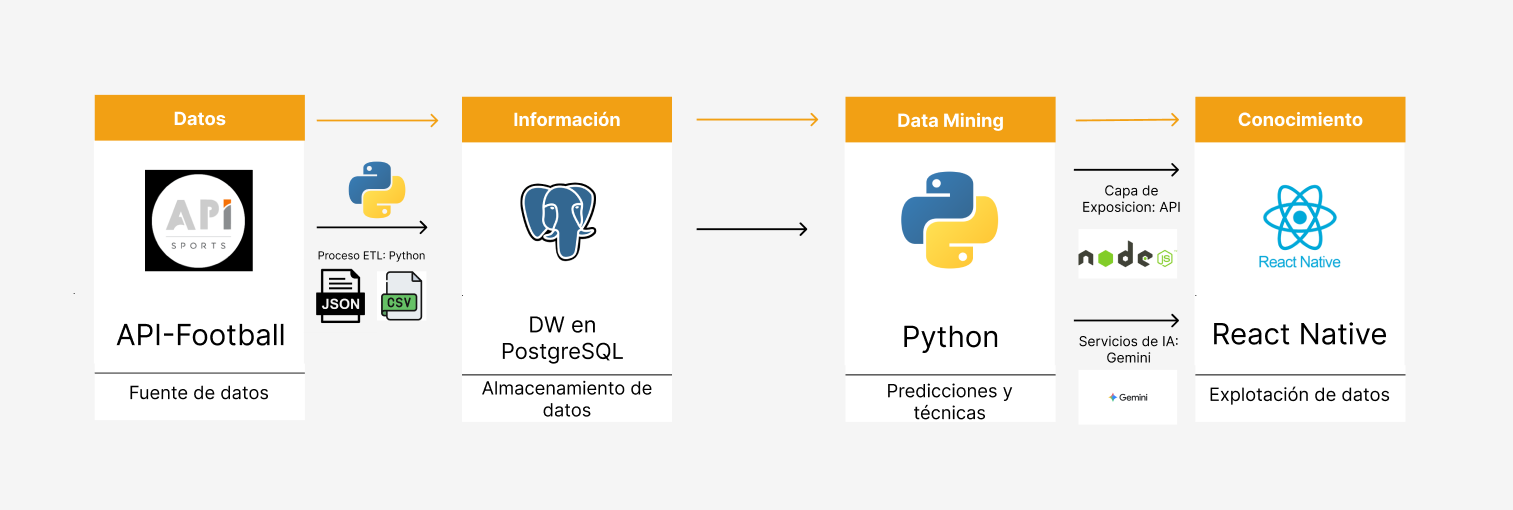
\includegraphics[width=1\linewidth]{figures/arquitectura_bi.png}
    \caption{Arquitectura BI.}
    \label{fig:arquitectura}
\end{figure}

\begin{itemize}
    \item Fuentes de datos (Ingesta): punto de entrada encargado de la extracción de información en bruto desde la API externa API-FOOTBALL en formato JSON.
    \item Proceso ETL: capa de procesamiento desarrollada en Python mediante las librerías pandas y numpy para la limpieza y transformación de archivos JSON a estructuras tabulares CSV.
    \item \textit{Data mining}: motor de analítica avanzada basado en scikit-learn donde se ejecutan los modelos de aprendizaje automático para la generación de métricas predictivas y los algoritmos de métricas estadísticas.
    \item Capa de información: almacén de datos centralizado en PostgreSQL, gestionado mediante DBeaver, que garantiza la persistencia e integridad de los datos procesados.
    \item Capa de exposicion (API): interfaz de servicios desarrollada en Node.js y
    Express, que actúa como puente de comunicación entre PostgreSQL, los servicios
    analíticos, el chatbot y el cliente móvil, y consulta entre el almacén de datos y el cliente.
    \item Servicios de IA: dentro de la capa backend se integran servicios avanzados como la API de Gemini, como el chatbot basado en IA generativa, que permite consultar la base de datos mediante preguntas en lenguaje natural, y el módulo de simulación, que ejecuta escenarios personalizados a partir de los resultados introducidos por el usuario.
    \item Explotación de datos: capa de presentación final desarrollada en React Native, encargada de la visualización de la información y los resultados del análisis para el usuario.
\end{itemize}

\subsection{Diseño físico de datos}

En esta sección se define la estructura física de datos que utilizará el sistema, a partir del modelo conceptual de clases, de manera que, teniendo presentes los requisitos establecidos para el sistema de información y las particularidades del entorno tecnológico, se consiga un acceso eficiente a los datos. La estructura física se compone de tablas, índices, procedimientos almacenados, secuencias y otros elementos dependientes del SGBD utilizado.

El diseño físico de la base de datos se ha planteado siguiendo un esquema en constelación, propio de entornos de \textit{data warehouse}. Este tipo de modelo se caracteriza por la existencia de varias tablas de hechos que comparten dimensiones comunes, permitiendo analizar la información desde distintas perspectivas. En el caso de este proyecto, las tablas de hechos almacenan métricas relacionadas con partidos, jugadores, equipos, temporadas y eventos, mientras que las tablas de dimensiones contienen información descriptiva como equipos, jugadores, partidos o tiempo. Esta organización facilita la realización de consultas analíticas, la generación de indicadores y la explotación posterior de los datos mediante técnicas de \textit{business intelligence} y \textit{data mining}.

Dentro de este modelo, las tablas de dimensiones representan entidades descriptivas del sistema y permiten contextualizar los datos almacenados. Por ejemplo, una dimensión puede contener información sobre un equipo, un jugador, un partido o una temporada. Por otro lado, las tablas de hechos almacenan datos cuantitativos o medibles, normalmente asociados a una o varias dimensiones. En este proyecto, estas tablas recogen estadísticas de rendimiento, resultados, eventos y métricas acumuladas, permitiendo analizar el comportamiento deportivo desde diferentes niveles de detalle.

\begin{figure}[H]
    \centering
    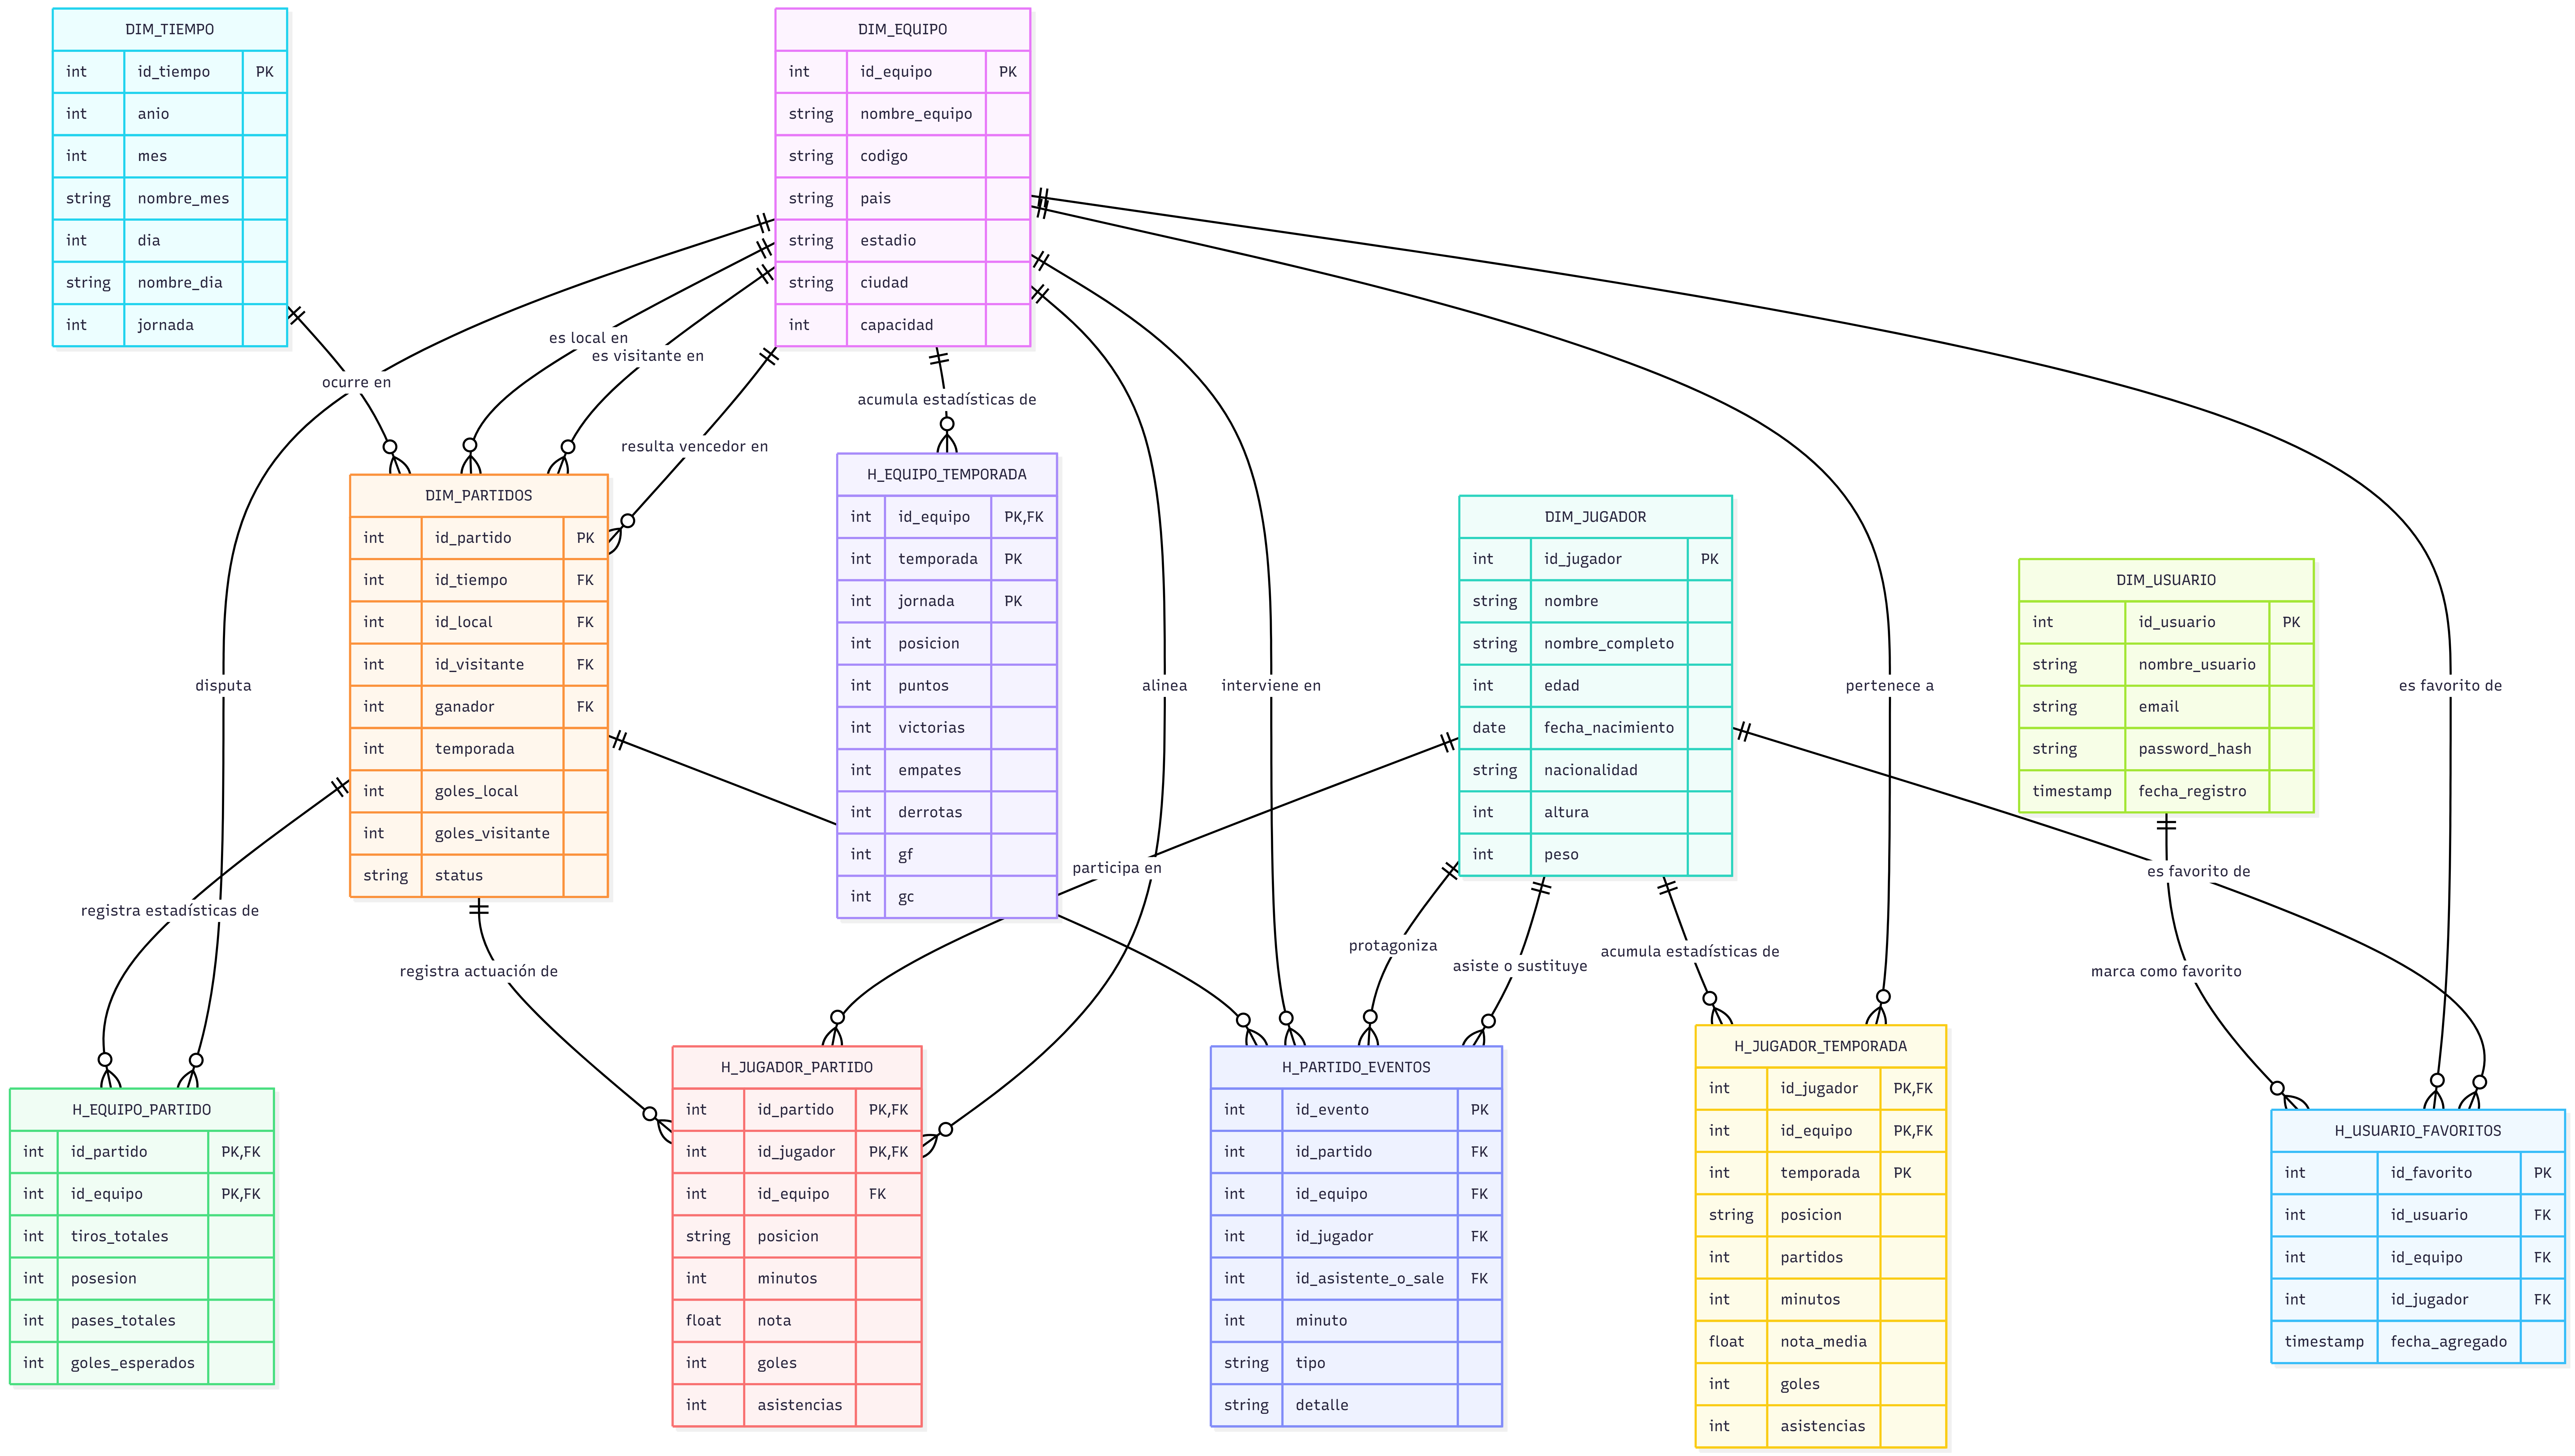
\includegraphics[width=1\linewidth]{figures/modelo_fisico.png}
    \caption{Modelo físico de la base de datos.}
    \label{fig:modelo_fisico}
\end{figure}

A continuación se describen las principales tablas que componen el modelo físico de datos. Para cada una de ellas se indican sus atributos más relevantes y su función dentro del sistema.
\subsubsection{Tablas de dimensión}

\begin{longtable}{|l|l|}
\caption{Atributos de la tabla dim\_equipo.} \\

\hline
\textbf{Atributo} & \textbf{Descripción} \\
\hline
\endfirsthead

\hline
\textbf{Atributo} & \textbf{Descripción} \\
\hline
\endhead

\hline
\multicolumn{2}{r}{\textit{Continúa en la siguiente página}} \\
\hline
\endfoot

\hline
\endlastfoot

id\_equipo & Identificador único del equipo. \\
nombre\_equipo & Nombre del equipo. \\
codigo & Código abreviado del equipo. \\
pais & País del equipo. \\
fundado\_en & Año de fundación.\\
logo & URL o ruta del escudo.\\
estadio & Nombre del estadio.\\
direccion & Dirección del estadio. \\
ciudad & Ciudad del equipo. \\
capacidad & Capacidad del estadio. \\
\hline

\end{longtable}

\begin{longtable}{|l|l|}
\caption{Atributos de la tabla dim\_jugador.} \\

\hline
\textbf{Atributo} & \textbf{Descripción} \\
\hline
\endfirsthead

\hline
\textbf{Atributo} & \textbf{Descripción} \\
\hline
\endhead

\hline
\multicolumn{2}{r}{\textit{Continúa en la siguiente página}} \\
\hline
\endfoot

\hline
\endlastfoot

id\_jugador & Identificador único del jugador. \\
nombre & Nombre deportivo del jugador. \\
nombre\_completo & Nombre completo del jugador. \\
edad & Edad del jugador. \\
fecha\_nacimiento & Fecha de nacimiento. \\
lugar\_nacimiento & Lugar de nacimiento. \\
pais\_nacimiento & País de nacimiento. \\
nacionalidad & Nacionalidad del jugador. \\
altura & Altura en centímetros. \\
peso & Peso en kilogramos. \\
foto & URL o ruta de la imagen del jugador. \\
\hline

\end{longtable}

\begin{longtable}{|l|l|}
\caption{Atributos de la tabla dim\_partidos.} \\

\hline
\textbf{Atributo} & \textbf{Descripción} \\
\hline
\endfirsthead

\hline
\textbf{Atributo} & \textbf{Descripción} \\
\hline
\endhead

\hline
\multicolumn{2}{r}{\textit{Continúa en la siguiente página}} \\
\hline
\endfoot

\hline
\endlastfoot

id\_partido & Identificador único del partido. \\
id\_tiempo & Referencia temporal del partido. \\
hora & Hora de disputa. \\
arbitro & Árbitro del encuentro. \\
estadio & Estadio del partido. \\
temporada & Temporada a la que pertenece. \\
id\_local & Equipo local. \\
id\_visitante & Equipo visitante. \\
ganador & Equipo ganador del partido. \\
goles\_local & Goles anotados por el local. \\
goles\_visitante & Goles anotados por el visitante. \\
status & Estado del partido. \\
\hline

\end{longtable}

\begin{longtable}{|l|l|}
\caption{Atributos de la tabla dim\_tiempo.} \\

\hline
\textbf{Atributo} & \textbf{Descripción} \\
\hline
\endfirsthead

\hline
\textbf{Atributo} & \textbf{Descripción} \\
\hline
\endhead

\hline
\multicolumn{2}{r}{\textit{Continúa en la siguiente página}} \\
\hline
\endfoot

\hline
\endlastfoot

id\_tiempo & Identificador temporal. \\
anio & Año. \\
mes & Número del mes. \\
nombre\_mes & Nombre del mes. \\
dia & Día del mes. \\
nombre\_dia & Nombre del día de la semana. \\
jornada & Jornada de la competición. \\
\hline

\end{longtable}

\subsubsection{Tablas de hechos}

\begin{longtable}{|l|l|}
\caption{Atributos de la tabla h\_equipo\_partido.} \\

\hline
\textbf{Atributo} & \textbf{Descripción} \\
\hline
\endfirsthead

\hline
\textbf{Atributo} & \textbf{Descripción} \\
\hline
\endhead

\hline
\multicolumn{2}{r}{\textit{Continúa en la siguiente página}} \\
\hline
\endfoot

\hline
\endlastfoot

id\_partido & Partido al que pertenecen las estadísticas. \\
id\_equipo & Equipo analizado. \\
tiros\_a\_puerta & Tiros realizados a portería. \\
tiros\_totales & Total de tiros. \\
tiros\_en\_area & Tiros realizados dentro del área. \\
tiros\_fuera\_area & Tiros realizados fuera del área. \\
faltas\_cometidas & Faltas realizadas. \\
corners & Saques de esquina. \\
fueras\_de\_juego & Fueras de juego. \\
posesion & Porcentaje de posesión. \\
tarjetas\_amarillas & Tarjetas amarillas recibidas. \\
tarjetas\_rojas & Tarjetas rojas recibidas. \\
paradas & Paradas realizadas. \\
pases\_totales & Total de pases. \\
pases\_acertados & Pases completados. \\
pct\_pases\_acertados & Porcentaje de acierto en pases. \\
goles\_esperados & Valor de goles esperados. \\
df\_goles\_esperados & Diferencia respecto a goles esperados. \\
\hline

\end{longtable}

\begin{longtable}{|l|l|}
\caption{Atributos de la tabla h\_equipo\_temporada.} \\

\hline
\textbf{Atributo} & \textbf{Descripción} \\
\hline
\endfirsthead

\hline
\textbf{Atributo} & \textbf{Descripción} \\
\hline
\endhead

\hline
\multicolumn{2}{r}{\textit{Continúa en la siguiente página}} \\
\hline
\endfoot

\hline
\endlastfoot

id\_equipo & Equipo al que pertenece el registro. \\
temporada & Temporada analizada. \\
jornada & Jornada correspondiente. \\
posicion & Posición en la clasificación. \\
nombre\_equipo & Nombre del equipo. \\
puntos & Puntos acumulados. \\
dg & Diferencia de goles. \\
forma & Racha reciente del equipo. \\
partidos\_jugados & Partidos disputados. \\
victorias & Victorias totales. \\
empates & Empates totales. \\
derrotas & Derrotas totales. \\
gf & Goles a favor. \\
gc & Goles en contra. \\
victorias\_local & Victorias como local. \\
empates\_local & Empates como local. \\
derrotas\_local & Derrotas como local. \\
victorias\_visitante & Victorias como visitante. \\
empates\_visitante & Empates como visitante. \\
derrotas\_visitante & Derrotas como visitante. \\
\hline

\end{longtable}

\begin{longtable}{|l|l|}
\caption{Atributos de la tabla h\_jugador\_partido.} \\

\hline
\textbf{Atributo} & \textbf{Descripción} \\
\hline
\endfirsthead

\hline
\textbf{Atributo} & \textbf{Descripción} \\
\hline
\endhead

\hline
\multicolumn{2}{r}{\textit{Continúa en la siguiente página}} \\
\hline
\endfoot

\hline
\endlastfoot

id\_partido & Partido disputado. \\
id\_jugador & Jugador analizado. \\
id\_equipo & Equipo del jugador. \\
posicion & Posición ocupada en el partido. \\
minutos & Minutos disputados. \\
nota & Valoración del jugador. \\
capitan & Indica si fue capitán. \\
sustituto & Indica si fue suplente. \\
goles & Goles anotados. \\
asistencias & Asistencias realizadas. \\
paradas & Paradas realizadas. \\
goles\_concedidos & Goles concedidos. \\
tiros\_totales & Tiros totales. \\
tiros\_a\_puerta & Tiros a puerta. \\
pases\_totales & Pases realizados. \\
pases\_clave & Pases clave. \\
precision\_pases & Precisión de pase. \\
regates & Regates completados. \\
duelos\_totales & Duelos disputados. \\
duelos\_ganados & Duelos ganados. \\
faltas\_cometidas & Faltas realizadas. \\
faltas\_recibidas & Faltas recibidas. \\
entradas & Entradas realizadas. \\
bloqueos & Bloqueos realizados. \\
intercepciones & Intercepciones realizadas. \\
amarilla & Tarjetas amarillas. \\
roja & Tarjetas rojas. \\
\hline

\end{longtable}

\begin{longtable}{|l|l|}
\caption{Atributos de la tabla h\_jugador\_temporada.} \\

\hline
\textbf{Atributo} & \textbf{Descripción} \\
\hline
\endfirsthead

\hline
\textbf{Atributo} & \textbf{Descripción} \\
\hline
\endhead

\hline
\multicolumn{2}{r}{\textit{Continúa en la siguiente página}} \\
\hline
\endfoot

\hline
\endlastfoot

id\_jugador & Jugador analizado. \\
id\_equipo & Equipo del jugador. \\
temporada & Temporada correspondiente. \\
posicion & Posición habitual del jugador. \\
partidos & Partidos disputados. \\
minutos & Minutos jugados. \\
titular & Partidos como titular. \\
nota\_media & Valoración media. \\
goles & Goles anotados. \\
asistencias & Asistencias realizadas. \\
tiros\_totales & Tiros totales. \\
tiros\_a\_puerta & Tiros a puerta. \\
pases\_totales & Pases realizados. \\
pases\_clave & Pases clave. \\
precision\_pases & Precisión de pase. \\
entradas & Entradas realizadas. \\
bloqueos & Bloqueos realizados. \\
intercepciones & Intercepciones realizadas. \\
duelos\_totales & Duelos disputados. \\
duelos\_ganados & Duelos ganados. \\
faltas\_sufridas & Faltas recibidas. \\
faltas\_cometidas & Faltas realizadas. \\
regates\_intentados & Regates intentados. \\
regates\_exito & Regates completados. \\
amarillas & Tarjetas amarillas. \\
rojas & Tarjetas rojas. \\
goles\_concedidos & Goles concedidos. \\
paradas & Paradas realizadas. \\
\hline

\end{longtable}

\begin{longtable}{|l|l|}
\caption{Atributos de la tabla h\_partido\_eventos.} \\

\hline
\textbf{Atributo} & \textbf{Descripción} \\
\hline
\endfirsthead

\hline
\textbf{Atributo} & \textbf{Descripción} \\
\hline
\endhead

\hline
\multicolumn{2}{r}{\textit{Continúa en la siguiente página}} \\
\hline
\endfoot

\hline
\endlastfoot

id\_evento & Identificador único del evento. \\
id\_partido & Partido en el que ocurre el evento. \\
minuto & Minuto del evento. \\
extra & Tiempo añadido. \\
id\_equipo & Equipo relacionado con el evento. \\
id\_jugador & Jugador protagonista del evento. \\
id\_asistente\_o\_sale & Jugador asistente o sustituido. \\
tipo & Tipo de evento. \\
detalle & Detalle del evento. \\
comentarios & Comentarios adicionales. \\
\hline

\end{longtable}

\subsubsection{Tablas de usuario}

\begin{longtable}{|l|l|}
\caption{Atributos de la tabla dim\_usuario.} \\

\hline
\textbf{Atributo} & \textbf{Descripción} \\
\hline
\endfirsthead

\hline
\textbf{Atributo} & \textbf{Descripción} \\
\hline
\endhead

\hline
\multicolumn{2}{r}{\textit{Continúa en la siguiente página}} \\
\hline
\endfoot

\hline
\endlastfoot

id\_usuario & Identificador único del usuario. \\
nombre\_usuario & Nombre de usuario. \\
email & Correo electrónico del usuario. \\
password\_hash & Contraseña cifrada. \\
fecha\_registro & Fecha de registro en el sistema. \\
\hline

\end{longtable}

\begin{longtable}{|l|l|}
\caption{Atributos de la tabla h\_usuario\_favoritos.} \\

\hline
\textbf{Atributo} & \textbf{Descripción} \\
\hline
\endfirsthead

\hline
\textbf{Atributo} & \textbf{Descripción} \\
\hline
\endhead

\hline
\multicolumn{2}{r}{\textit{Continúa en la siguiente página}} \\
\hline
\endfoot

\hline
\endlastfoot

id\_favorito & Identificador único del favorito. \\
id\_usuario & Usuario que guarda el favorito. \\
id\_equipo & Equipo marcado como favorito. \\
id\_jugador & Jugador marcado como favorito. \\
fecha\_agregado & Fecha en la que se añadió el favorito. \\
\hline

\end{longtable}

\subsection{Diseño de tablas de \textit{data mining}}

Los algoritmos de minería de datos desarrollados en este trabajo generan una serie de tablas auxiliares que almacenan los resultados obtenidos por cada técnica de análisis. Estas tablas no forman parte del modelo conceptual principal del sistema, sino que constituyen una capa analítica utilizada por la aplicación para mostrar predicciones, simulaciones e indicadores avanzados.

Cada tabla es generada automáticamente mediante scripts desarrollados en Python, cuyos resultados son posteriormente almacenados en la base de datos PostgreSQL para ser consumidos por la API y la aplicación móvil.

\renewcommand{\arraystretch}{1.2}
\begin{longtable}{|p{4cm}|p{3cm}|p{2.2cm}|p{5cm}|}
\caption{Diseño de las tablas de \textit{data mining} implementadas.}
\label{tab:tablas_dm} \\

\hline
\textbf{Tabla} & \textbf{Algoritmo} & \textbf{Clave primaria} & \textbf{Descripción} \\
\hline
\endfirsthead

\hline
\textbf{Tabla} & \textbf{Algoritmo} & \textbf{Clave primaria} & \textbf{Descripción} \\
\hline
\endhead

\hline
\multicolumn{4}{r}{\textit{Continúa en la siguiente página}} \\
\hline
\endfoot

\hline
\endlastfoot

\path{dm_estado_forma_jugadores} &
Índice de forma &
\texttt{id\_jugador} &
Almacena el estado de forma actual de cada jugador y su evolución reciente. \\
\hline

\path{dm_estado_forma_equipos} &
Índice de forma &
\texttt{id\_equipo} &
Almacena el estado de forma actual de cada equipo junto con indicadores de tendencia y variabilidad. \\
\hline

\path{dm_perfil_estadistico_jugadores} &
Métricas estadísticas &
\texttt{id\_jugador, temporada} &
Contiene el perfil estadístico de cada jugador en distintas dimensiones del juego. \\
\hline

\path{dm_necesidades_plantilla} &
Reglas heurísticas &
\texttt{id\_equipo, temporada, necesidad} &
Recoge las necesidades detectadas en la plantilla de cada equipo y la causa que las justifica. \\
\hline

\path{dm_recomendacion_fichajes} &
Reglas heurísticas &
\texttt{id\_equipo, id\_jugador, necesidad} &
Acosia las necesidades de cada equipo en la temporada actual con jugadores que encajen con lo que buscan, generando una recomendación por necesidad. \\
\hline

\path{dm_probables_goleadores} &
Cálculo heurístico &
\texttt{id\_partido, id\_jugador} &
Contiene los jugadores con mayor probabilidad de marcar en cada partido. \\
\hline

\path{dm_prediccion_partidos} &
SVM &
\texttt{id\_partido} &
Almacena las probabilidades de victoria local, empate y victoria visitante para cada partido pendiente. \\
\hline

\path{dm_simulacion_montecarlo} &
Monte Carlo &
\texttt{id\_equipo} &
Guarda las probabilidades de campeón, clasificación europea, permanencia y descenso de cada equipo. \\
\hline

\path{dm_similitud_jugadores} &
K-means &
\texttt{id\_jugador, temporada} &
Agrupa a los jugadores según la similitud de sus características estadísticas e identifica los cinco jugadores más parecidos. \\
\hline

\path{dm_golesesperados_partidos} &
Random Forest Regressor &
\texttt{id\_partido} &
Almacena el número estimado de goles que marcará cada equipo en un partido. \\
\hline

\end{longtable}
\subsection{Diseño de la interfaz de usuario} 
En esta sección se presenta el diseño visual final de la aplicación, describiendo la organización de las pantallas, la distribución de los elementos de la interfaz y las decisiones tomadas en relación con la identidad visual del sistema. Además, se detallan aspectos como el logotipo, la paleta de colores y el nombre de la aplicación, con el objetivo de mostrar cómo se ha construido una interfaz coherente, intuitiva y adaptada al contexto de una aplicación de análisis futbolístico.
\subsection{Diseño final}

El diseño final de la aplicación mantiene la idea inicial de ofrecer una herramienta visual e intuitiva para consultar información relacionada con LaLiga, aunque durante el desarrollo se incorporaron nuevas funcionalidades que hicieron necesario adaptar varias pantallas. En la versión final no solo se permite consultar equipos, jugadores, partidos y temporadas, sino también acceder a análisis estadísticos, simulaciones, predicciones y consultas mediante inteligencia artificial.

La interfaz se ha organizado para facilitar la navegación entre las distintas secciones principales de la aplicación. Para ello se utilizaron vistas diferenciadas para el acceso de usuarios, la consulta de información deportiva, las funcionalidades avanzadas y la configuración. Además, se incorporó soporte para tema claro y tema oscuro.

La navegación principal se realiza mediante un menú desde el que el usuario puede acceder a las diferentes funcionalidades, junto con un buscador que facilita la localización de información dentro del sistema.

\begin{figure}[H]
\centering
\begin{subfigure}[b]{0.4\textwidth}
\centering
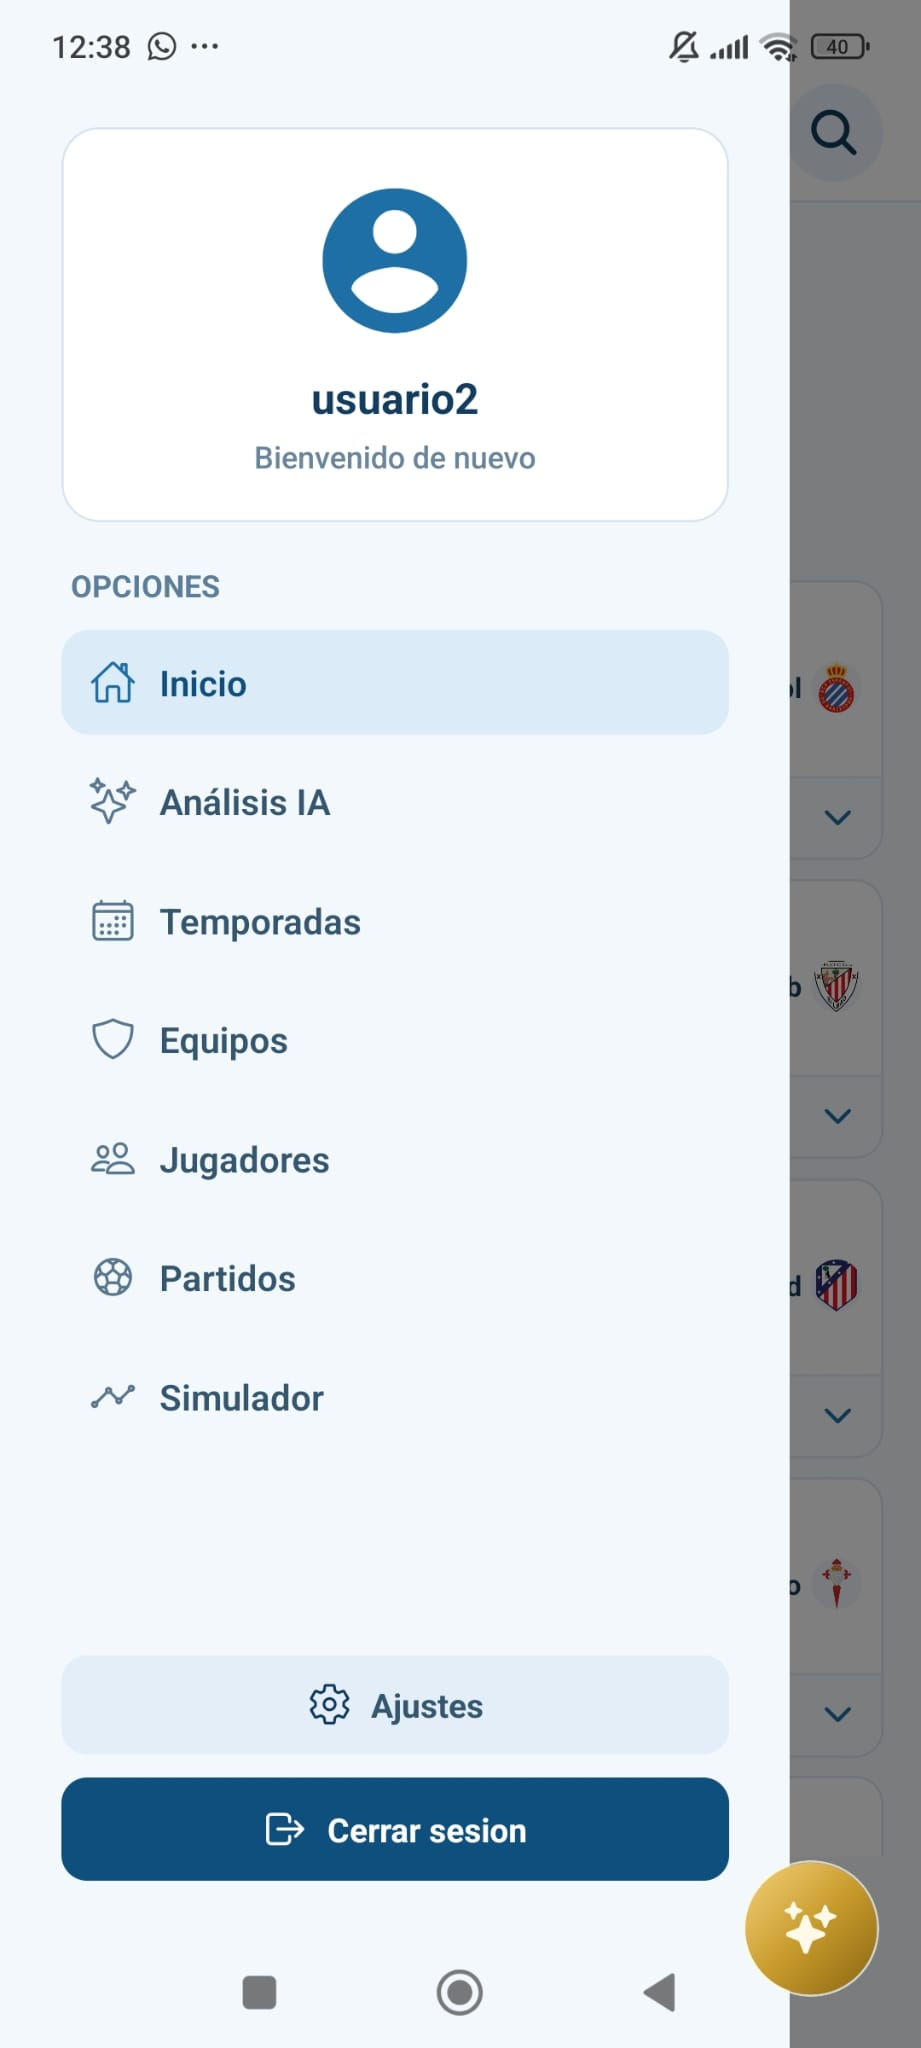
\includegraphics[width=0.5\textwidth]{figures/cap_menu.jpeg}
\caption{Menú principal}
\label{fig:menu}
\end{subfigure}
%
\begin{subfigure}[b]{0.4\textwidth}
\centering
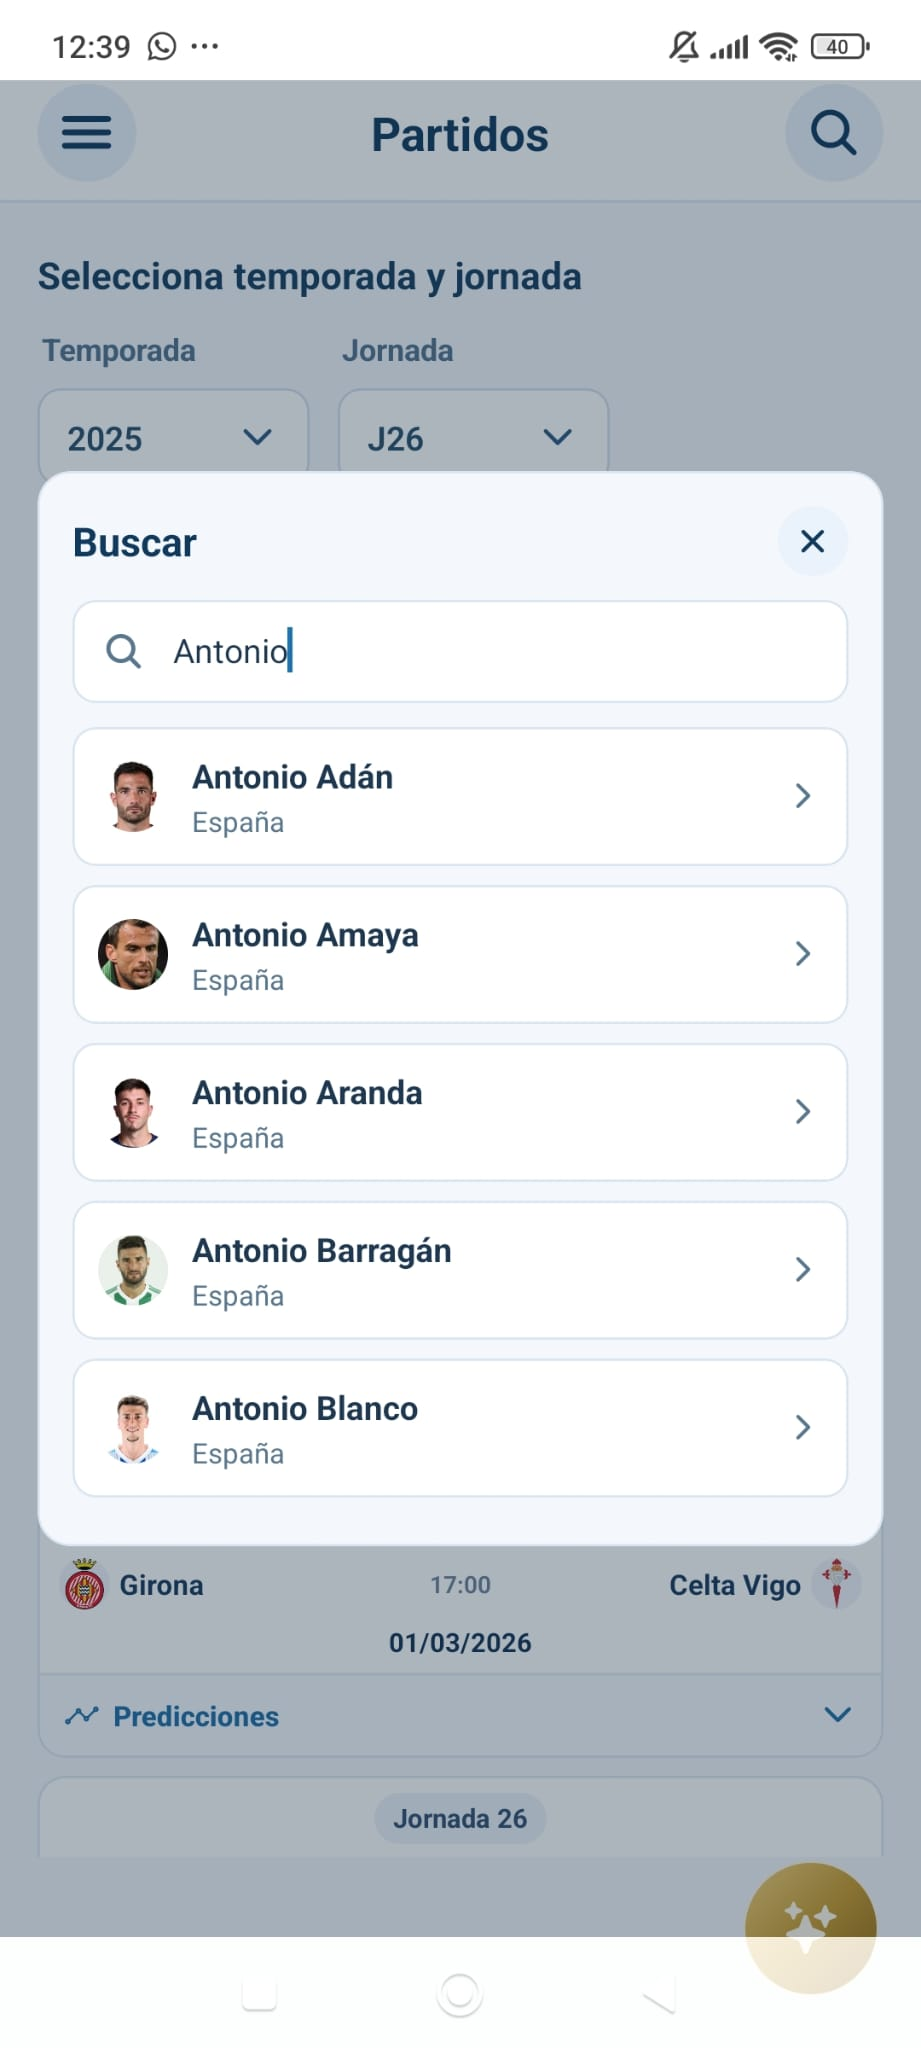
\includegraphics[width=0.5\textwidth]{figures/cap_buscador.jpeg}
\caption{Buscador}
\label{fig:buscador}
\end{subfigure}
\caption{Navegación y búsqueda dentro de la aplicación}
\label{fig:menu_buscador}
\end{figure}

Las pantallas de acceso y gestión de usuario permiten iniciar sesión, registrar una nueva cuenta y consultar o modificar los datos del perfil.

\begin{figure}[H]
\centering
\begin{subfigure}[b]{0.32\textwidth}
\centering
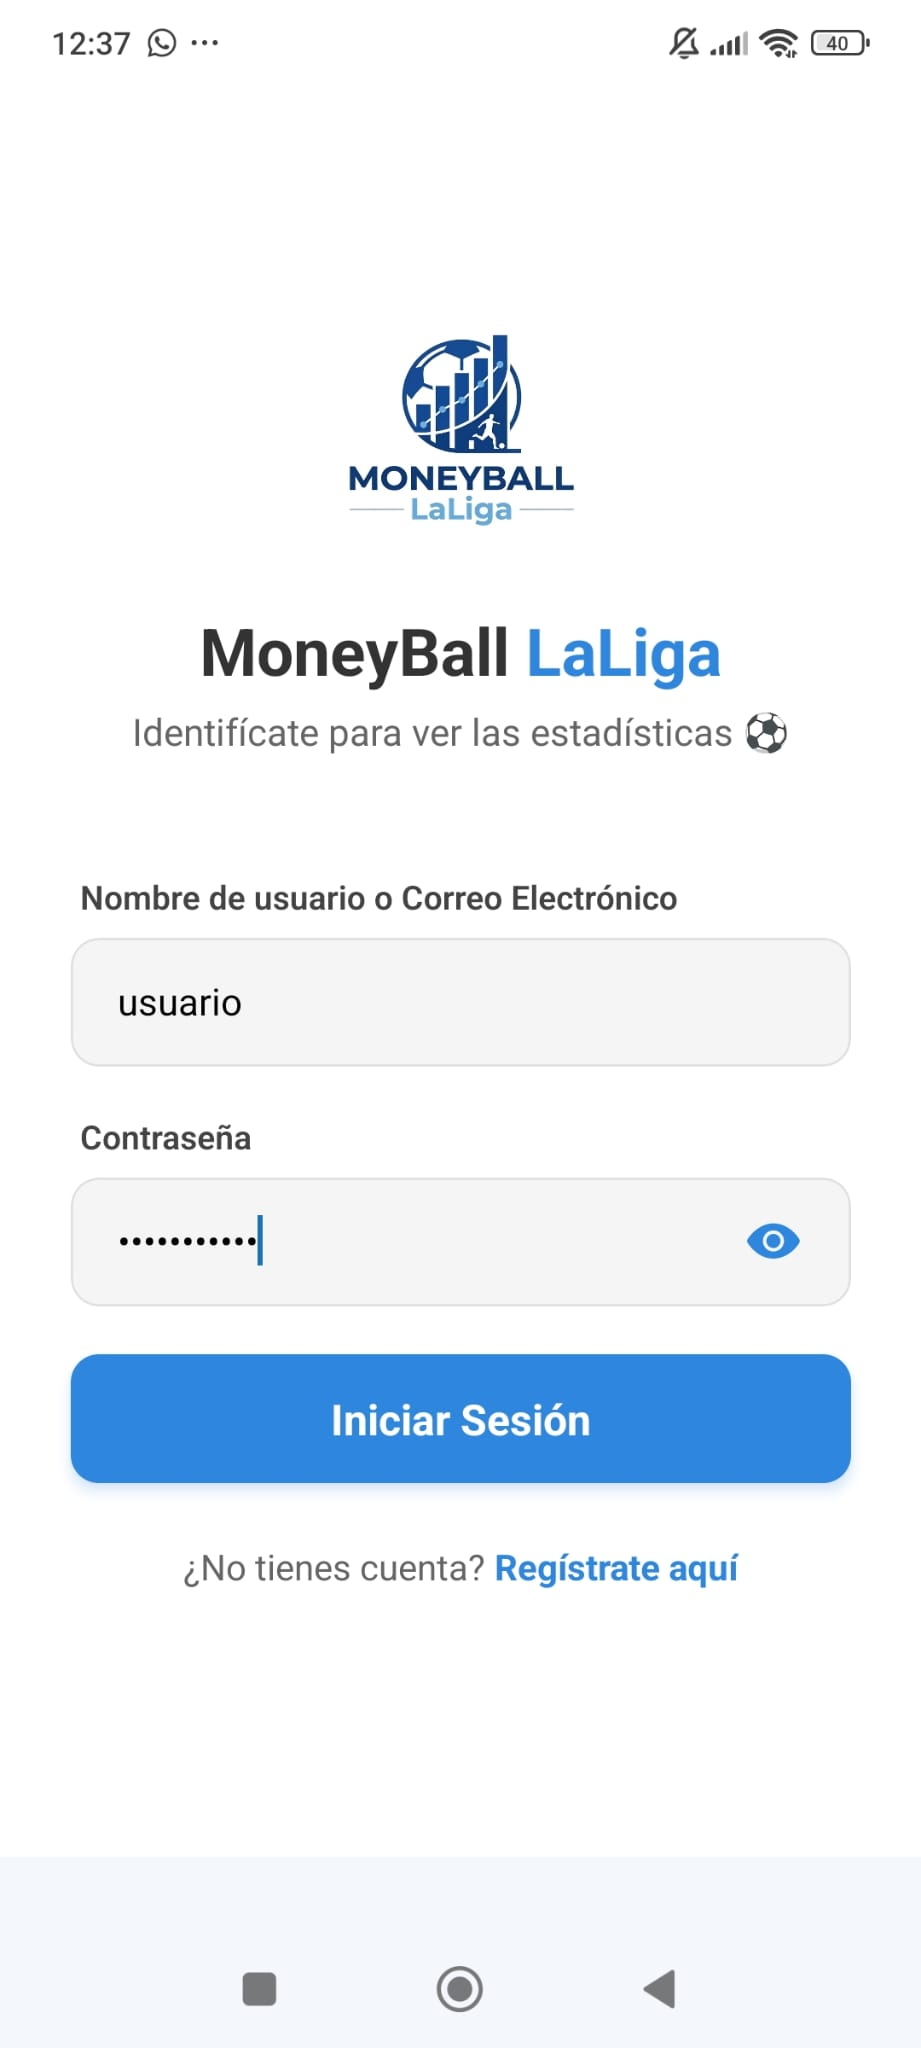
\includegraphics[width=0.8\textwidth]{figures/cap_iniciosesion.jpeg}
\caption{Inicio de sesión}
\label{fig:inicio_sesion}
\end{subfigure}
\hfill
\begin{subfigure}[b]{0.32\textwidth}
\centering
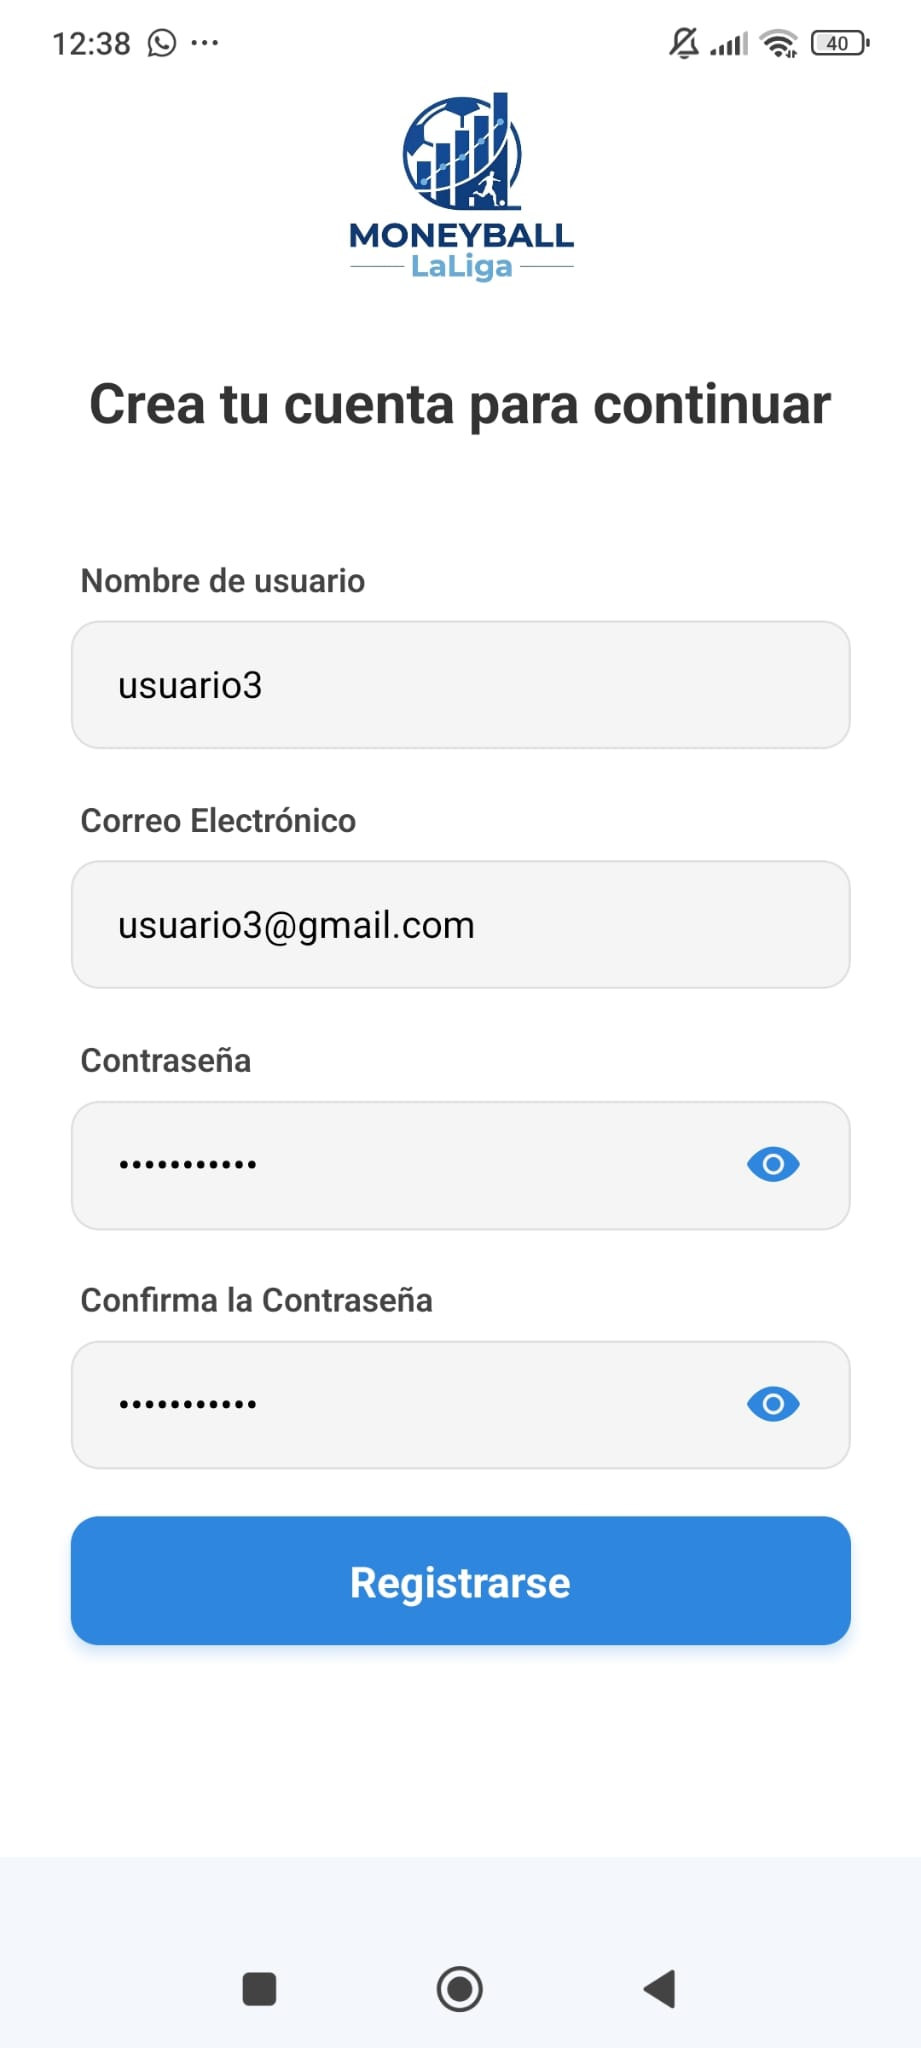
\includegraphics[width=0.8\textwidth]{figures/cap_registro.jpeg}
\caption{Registro}
\label{fig:registro}
\end{subfigure}
\hfill
\begin{subfigure}[b]{0.32\textwidth}
\centering
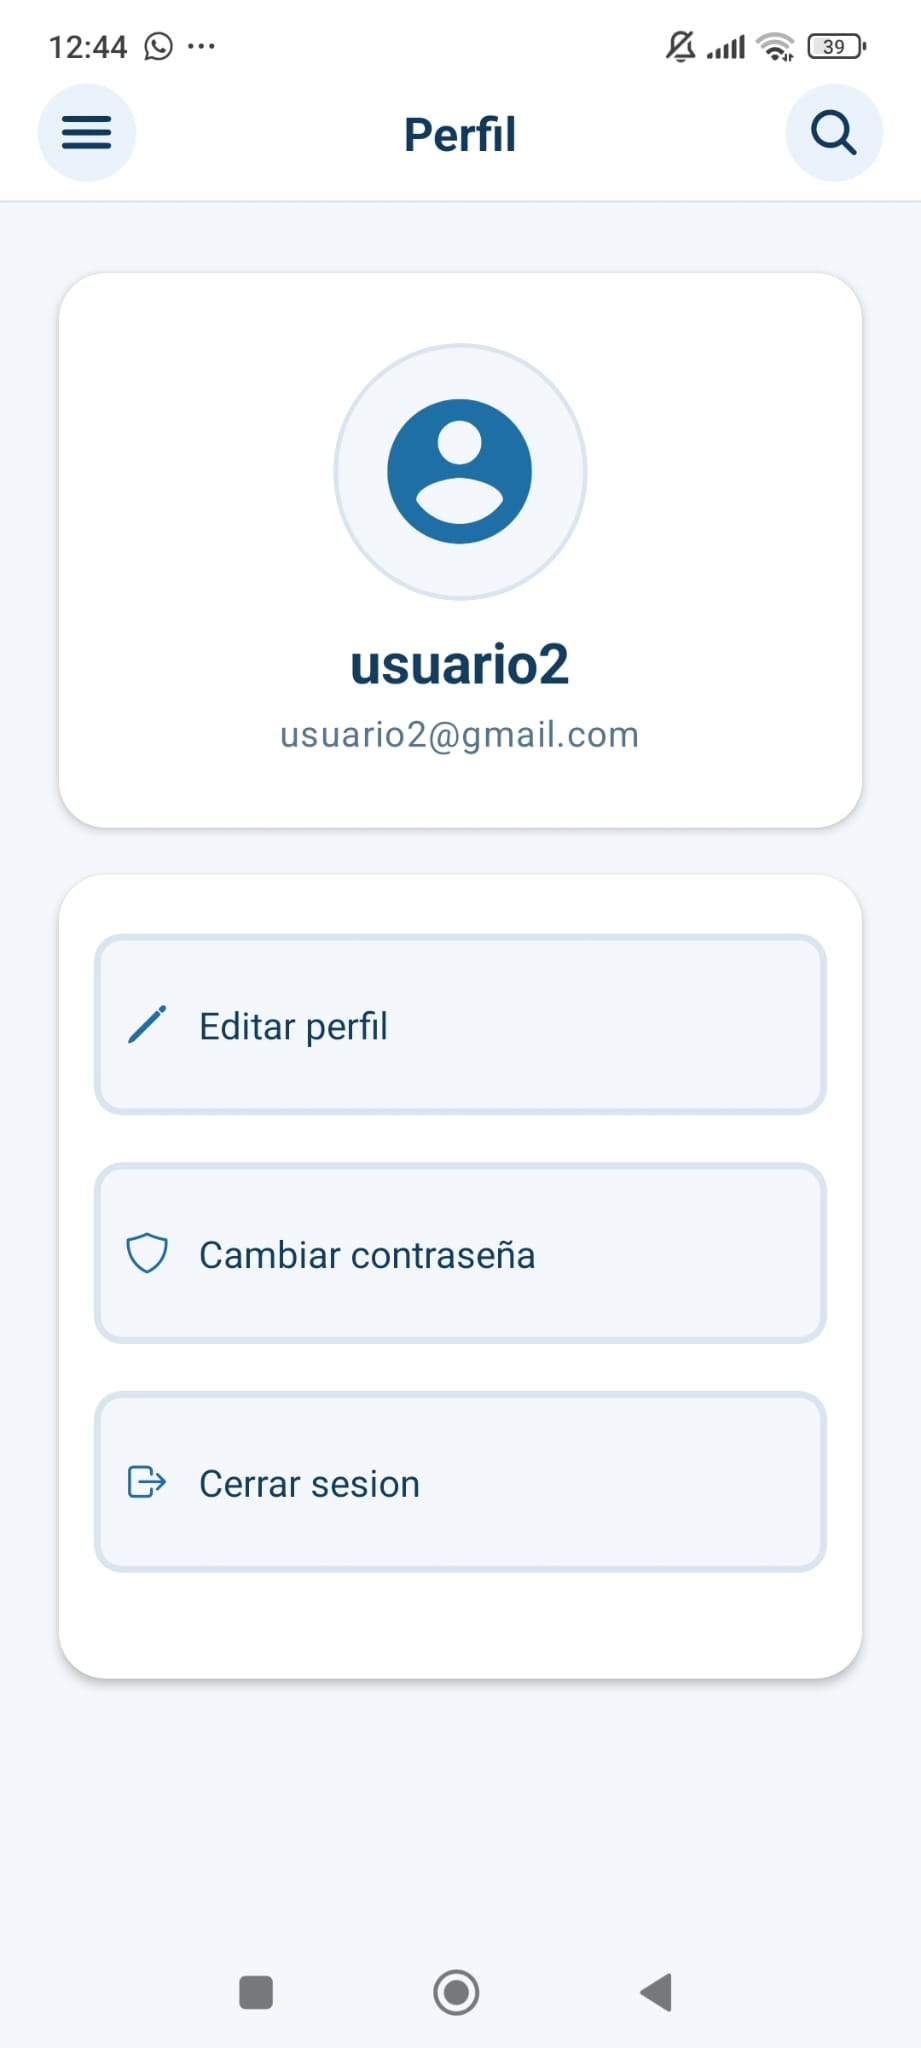
\includegraphics[width=0.8\textwidth]{figures/cap_perfil.jpeg}
\caption{Perfil}
\label{fig:perfil}
\end{subfigure}

\caption{Pantallas de acceso y gestión del usuario}
\label{fig:gestion_usuario}
\end{figure}

Las principales pantallas de consulta deportiva permiten acceder a jugadores, partidos y temporadas. Desde estas vistas se puede explorar la información almacenada en la base de datos y consultar estadísticas, eventos, clasificaciones y otros datos relevantes.

\begin{figure}[H]
\centering
\begin{subfigure}[b]{0.32\textwidth}
\centering
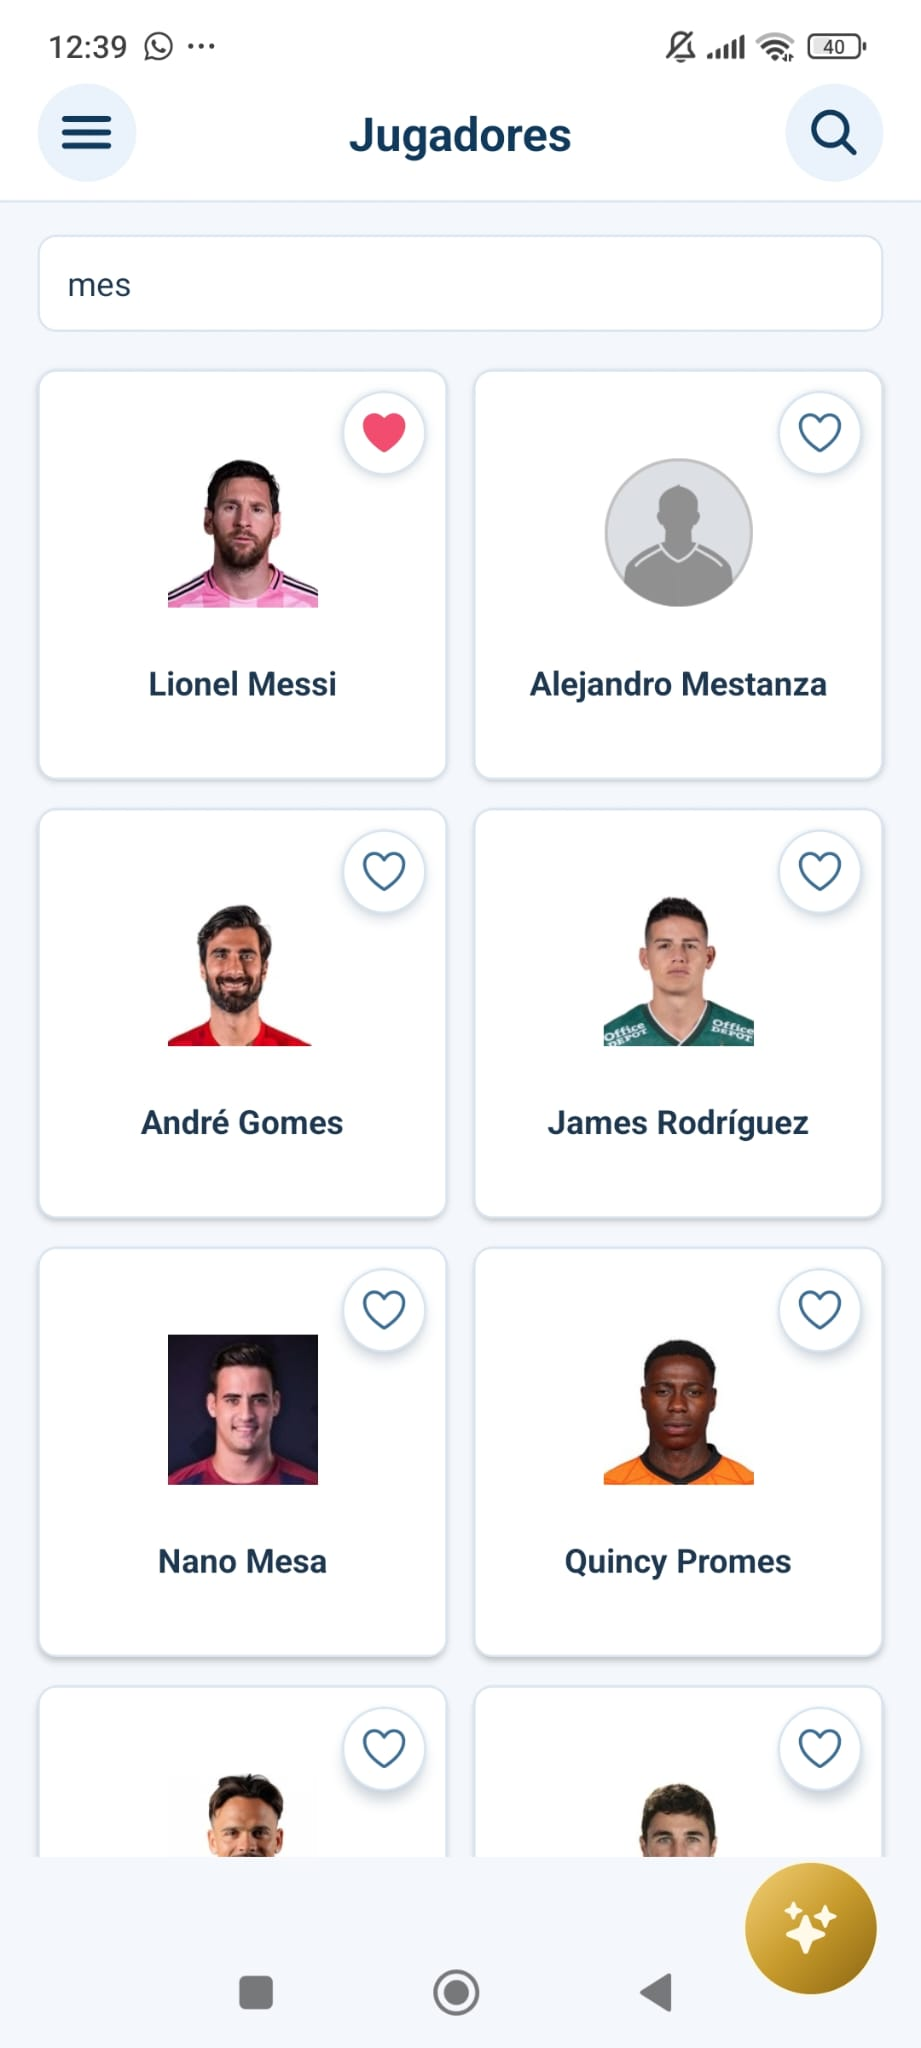
\includegraphics[width=0.8\textwidth]{figures/cap_jugadores.jpeg}
\caption{Jugadores}
\label{fig:jugadores}
\end{subfigure}
\hfill
\begin{subfigure}[b]{0.32\textwidth}
\centering
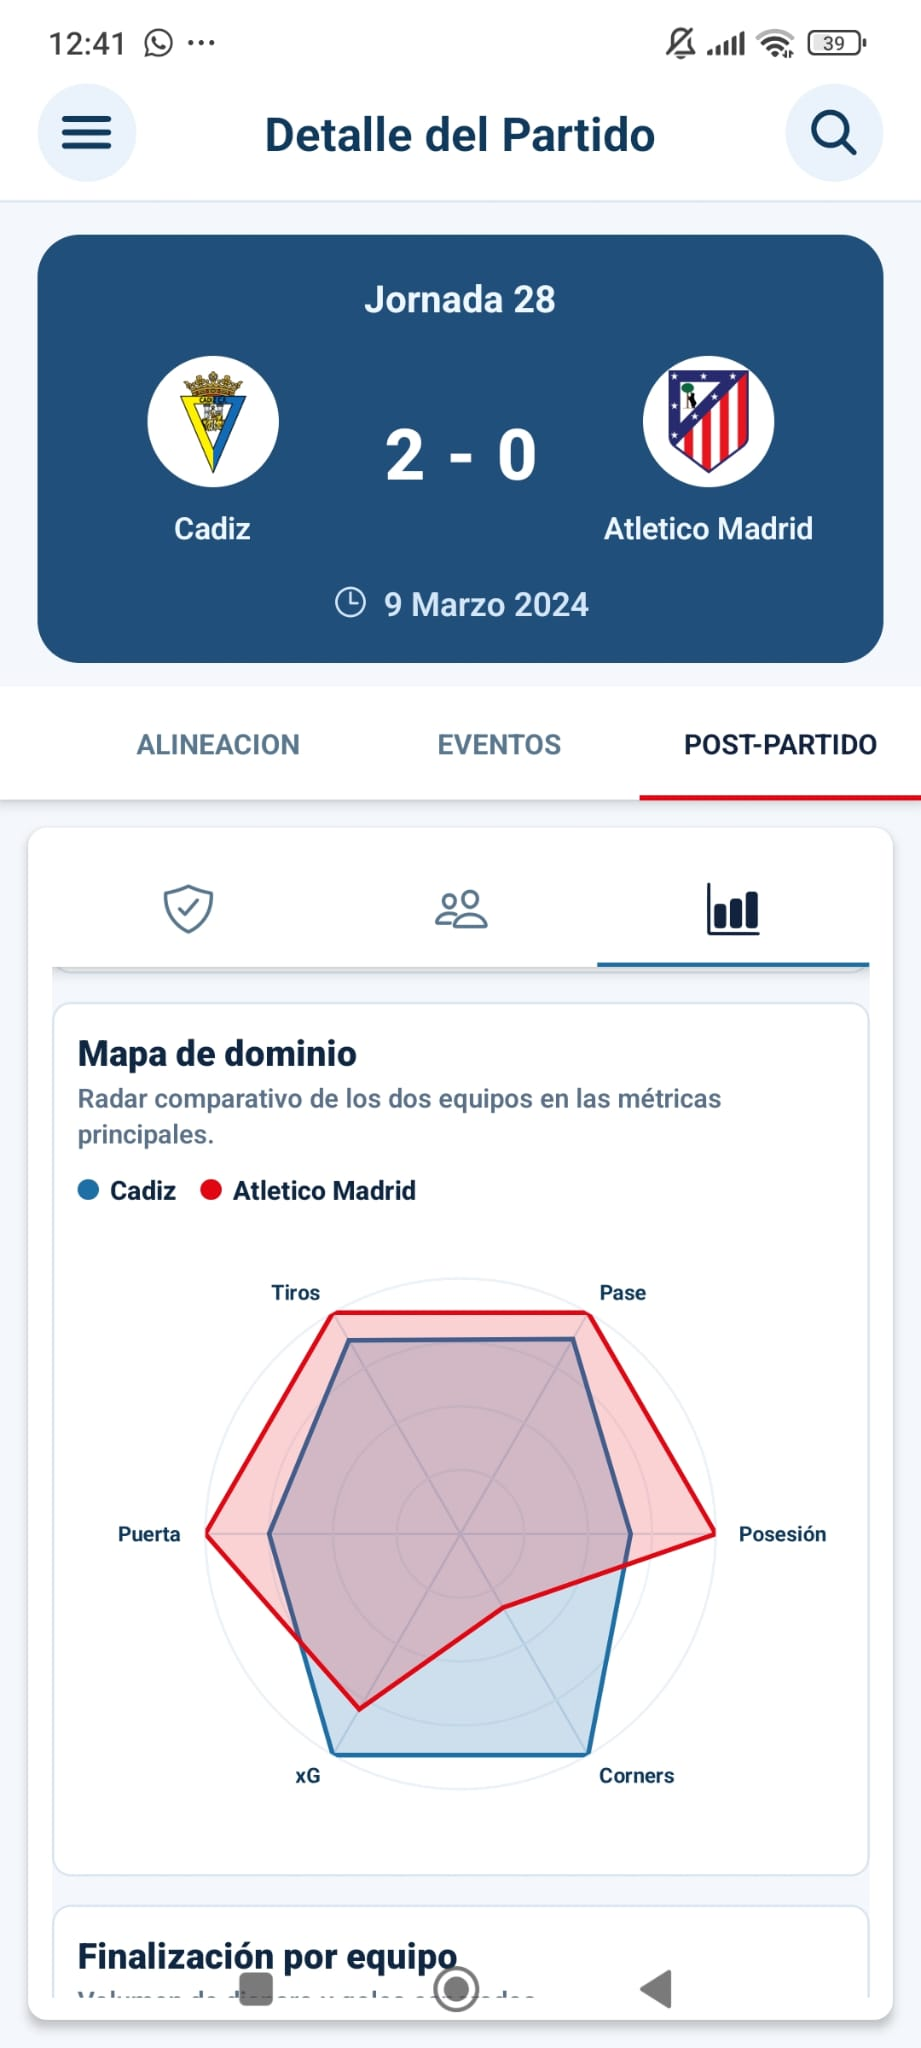
\includegraphics[width=0.8\textwidth]{figures/cap_dash_partido.jpeg}
\caption{Partido}
\label{fig:dashboard_partido}
\end{subfigure}
\hfill
\begin{subfigure}[b]{0.32\textwidth}
\centering
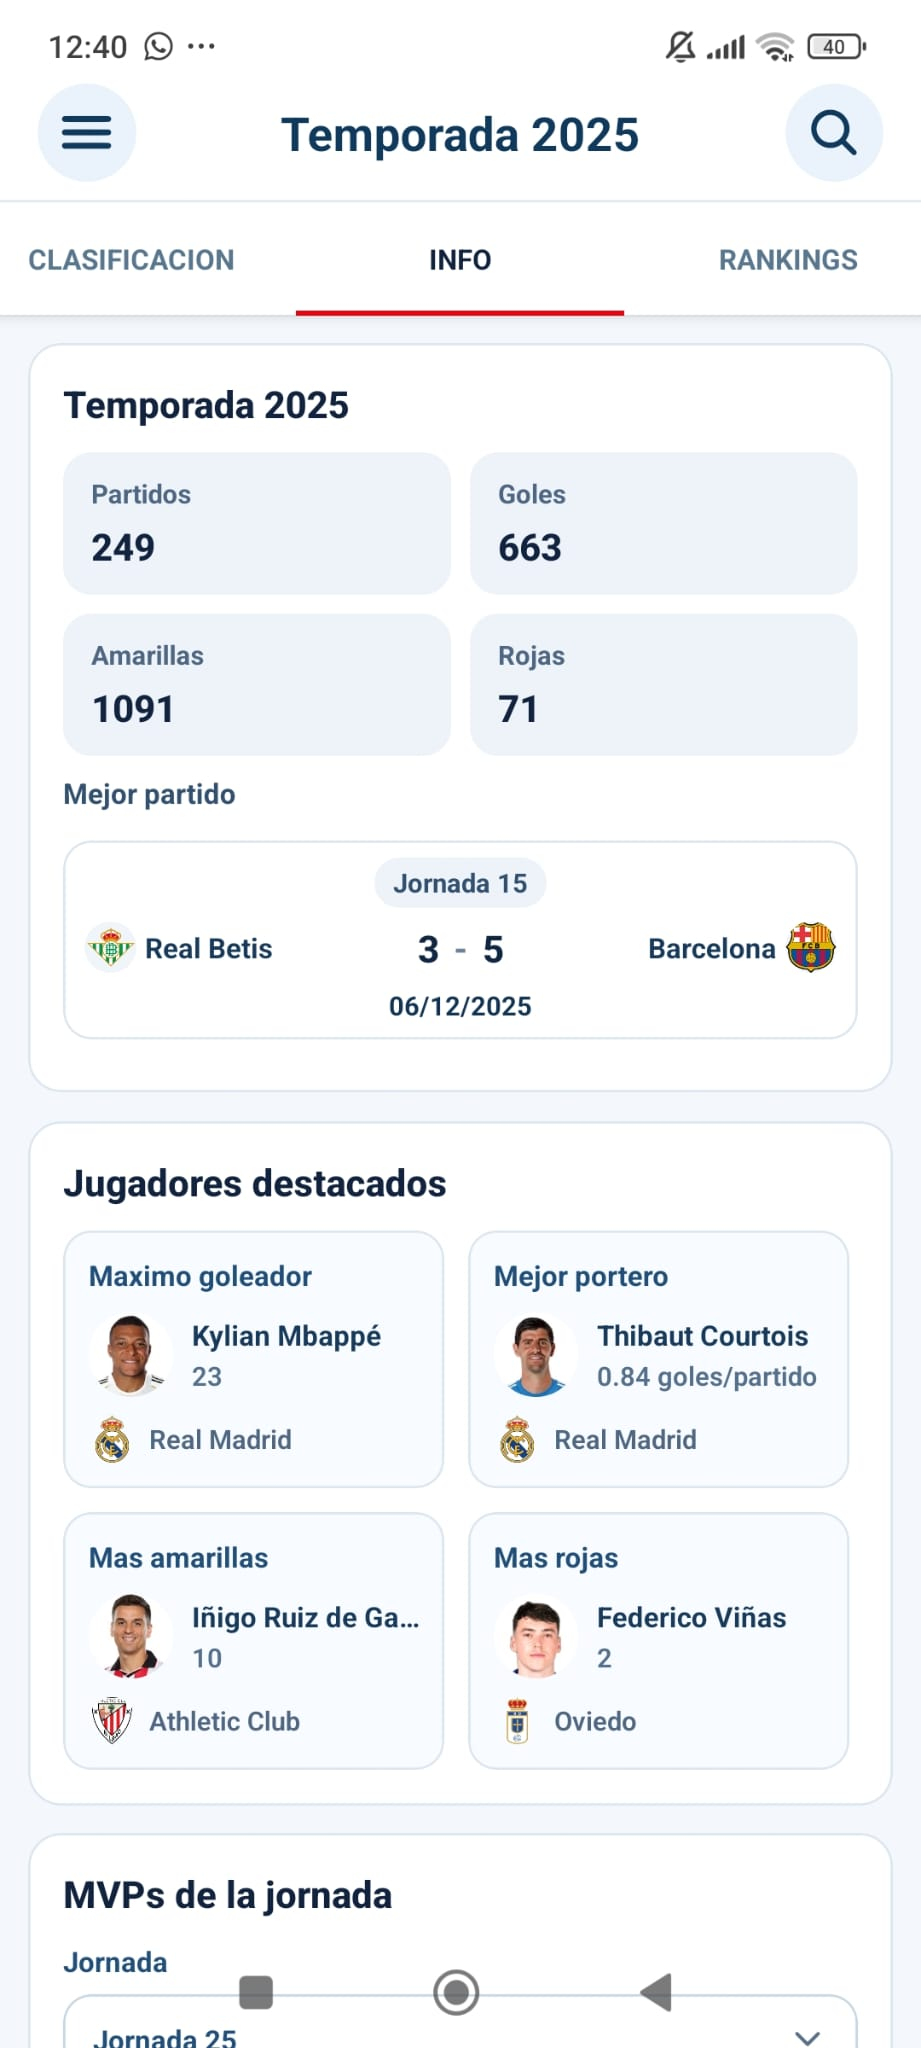
\includegraphics[width=0.8\textwidth]{figures/cap_tempo_inof.jpeg}
\caption{Temporada}
\label{fig:temporada}
\end{subfigure}

\caption{Principales pantallas de consulta deportiva}
\label{fig:consultas_deportivas}
\end{figure}

Entre las funcionalidades avanzadas se encuentran el análisis mediante inteligencia artificial y la simulación de temporadas. El módulo de inteligencia artificial permite generar información procesada a partir de los datos disponibles y guardar determinados análisis como favoritos.

\begin{figure}[H]
\centering
\begin{subfigure}[b]{0.4\textwidth}
\centering
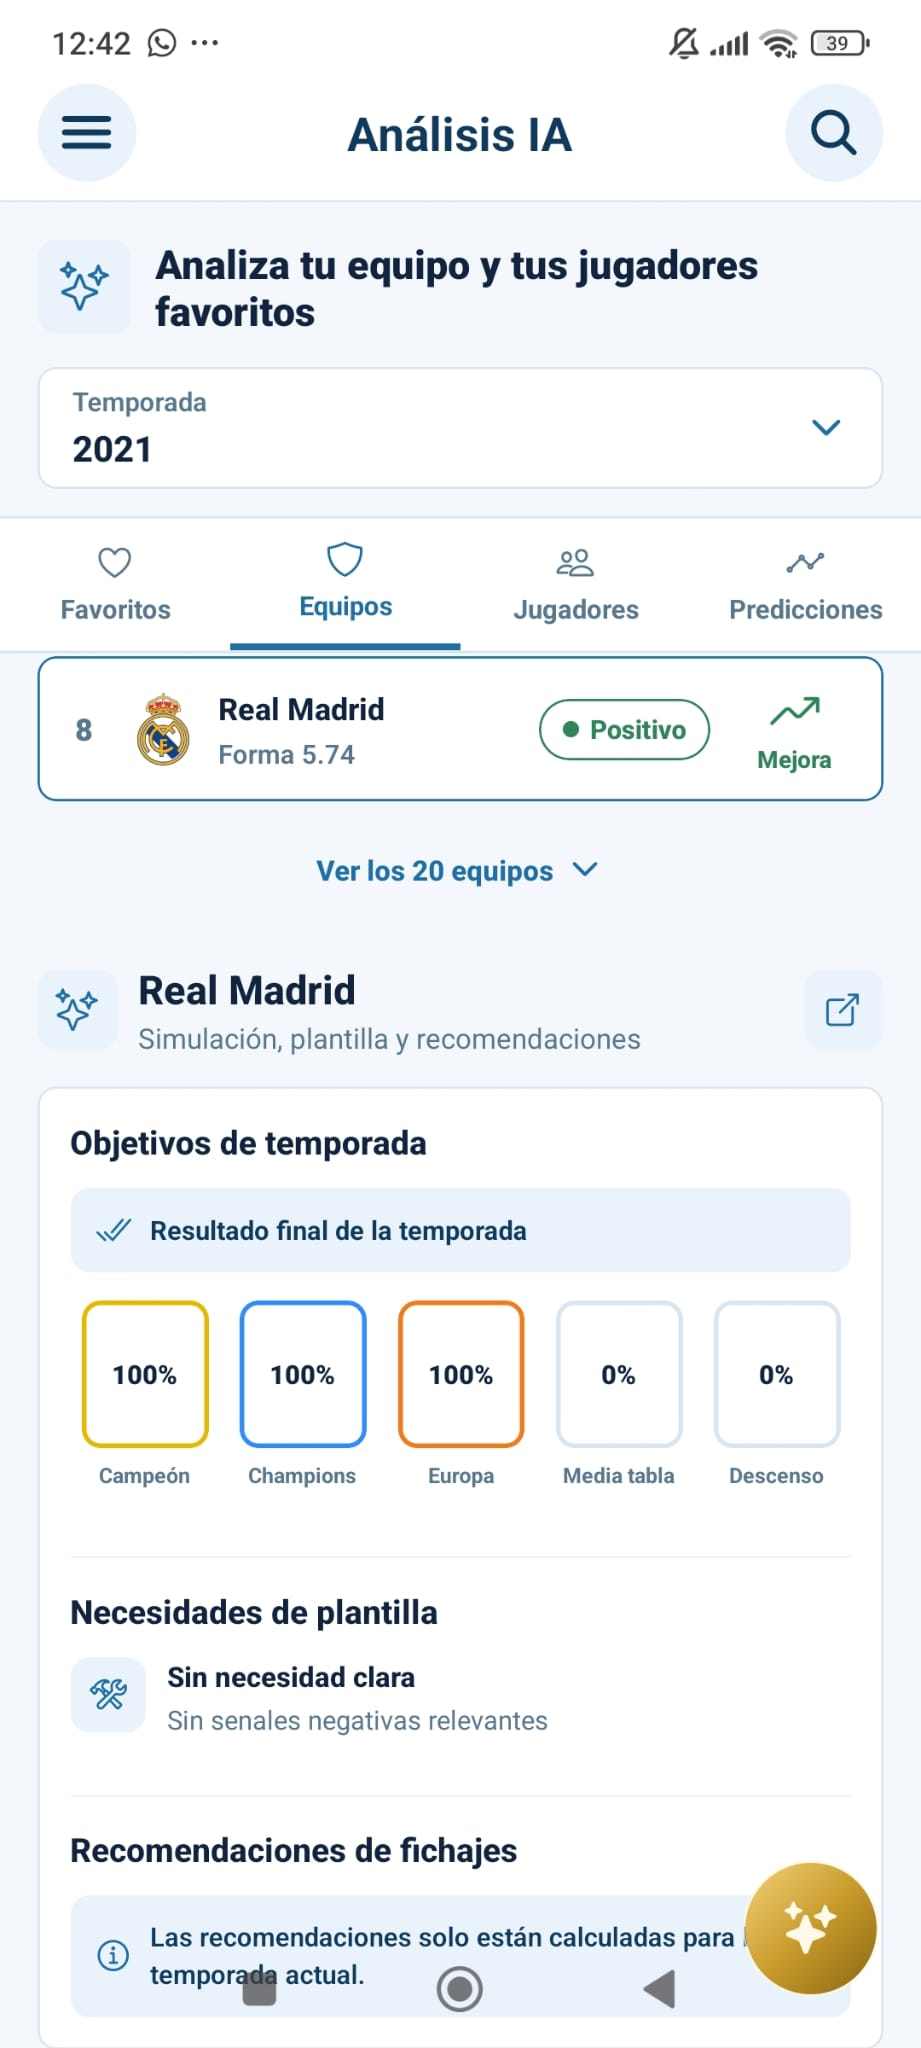
\includegraphics[width=0.5\textwidth]{figures/cap_analisisIA.jpeg}
\caption{Análisis mediante IA}
\label{fig:analisis_ia}
\end{subfigure}
%
\begin{subfigure}[b]{0.4\textwidth}
\centering
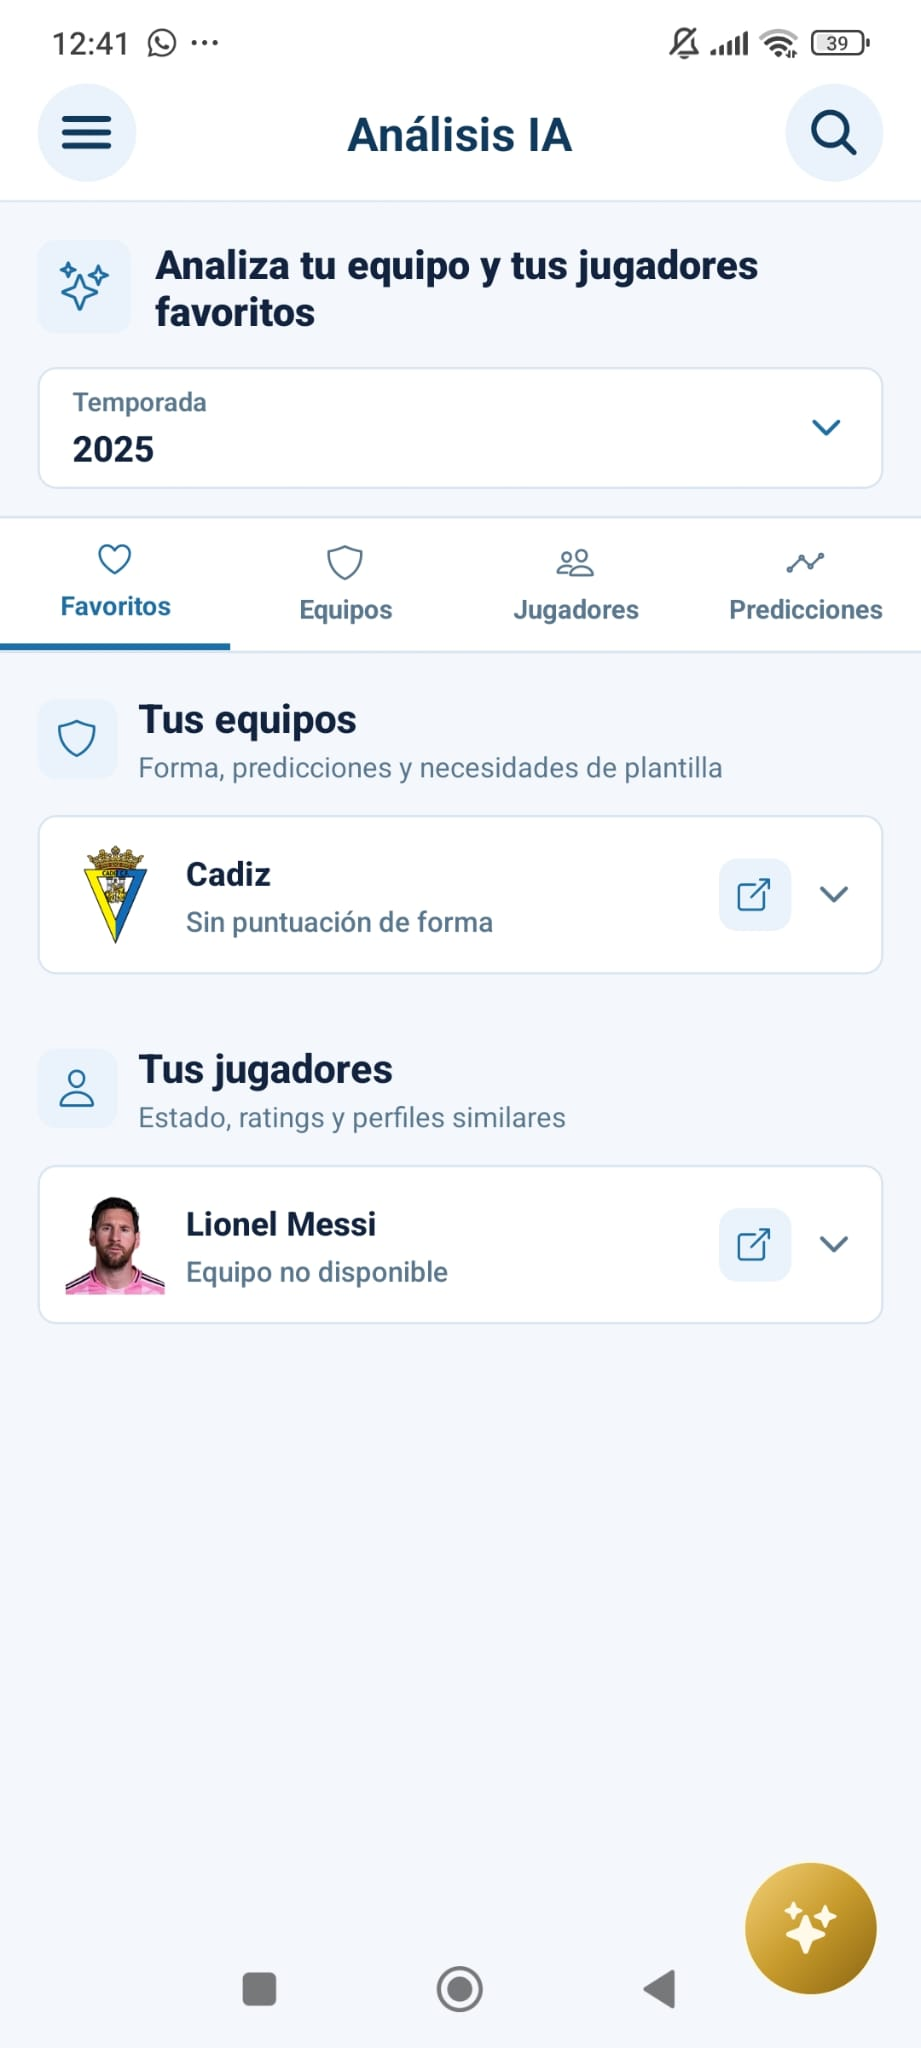
\includegraphics[width=0.5\textwidth]{figures/cap_analisisIA_Fav.jpeg}
\caption{Análisis guardado como favorito}
\label{fig:analisis_ia_fav}
\end{subfigure}
\caption{Funcionalidades de análisis mediante inteligencia artificial}
\label{fig:analisis_ia_general}
\end{figure}

La simulación permite analizar posibles escenarios futuros de la competición mediante el cálculo de probabilidades y la ejecución de simulaciones. El usuario puede consultar tanto la clasificación simulada como las probabilidades empleadas y los resultados finales obtenidos.

\begin{figure}[H]
\centering
\begin{subfigure}[b]{0.32\textwidth}
\centering
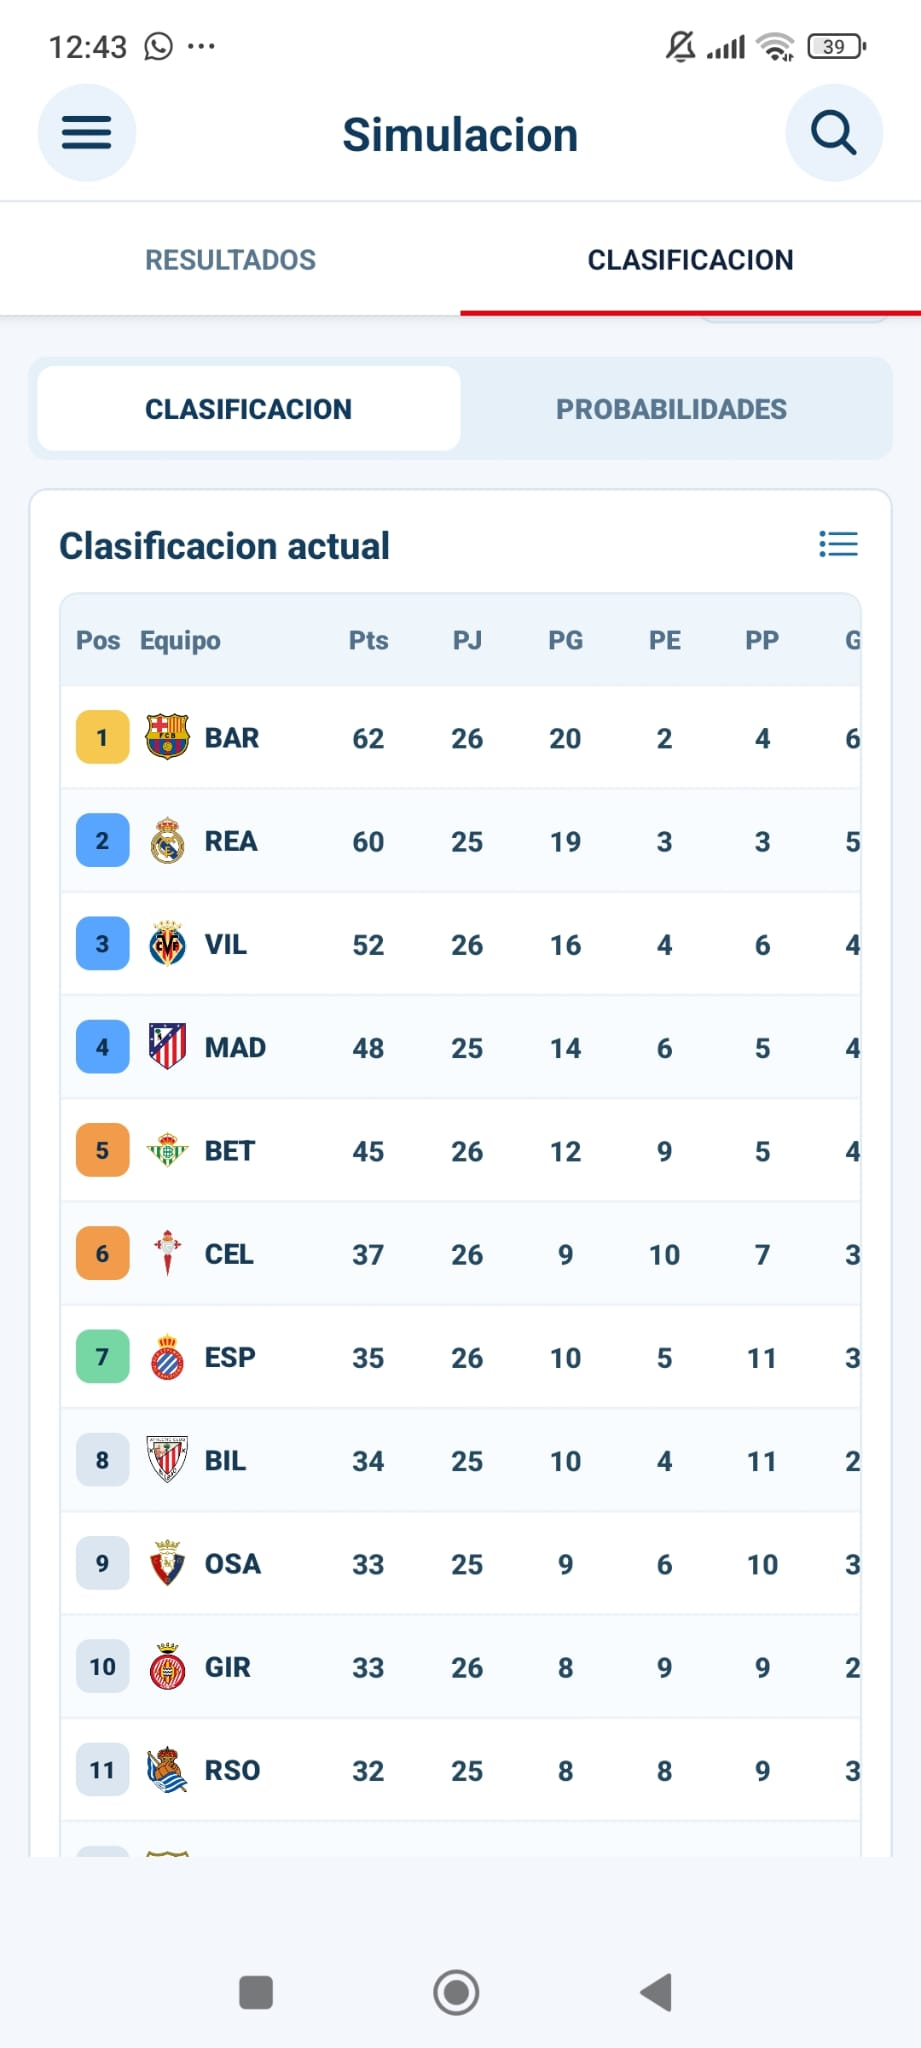
\includegraphics[width=0.8\textwidth]{figures/cap_sim_clasi.jpeg}
\caption{Clasificación simulada}
\label{fig:sim_clasi}
\end{subfigure}
\hfill
\begin{subfigure}[b]{0.32\textwidth}
\centering
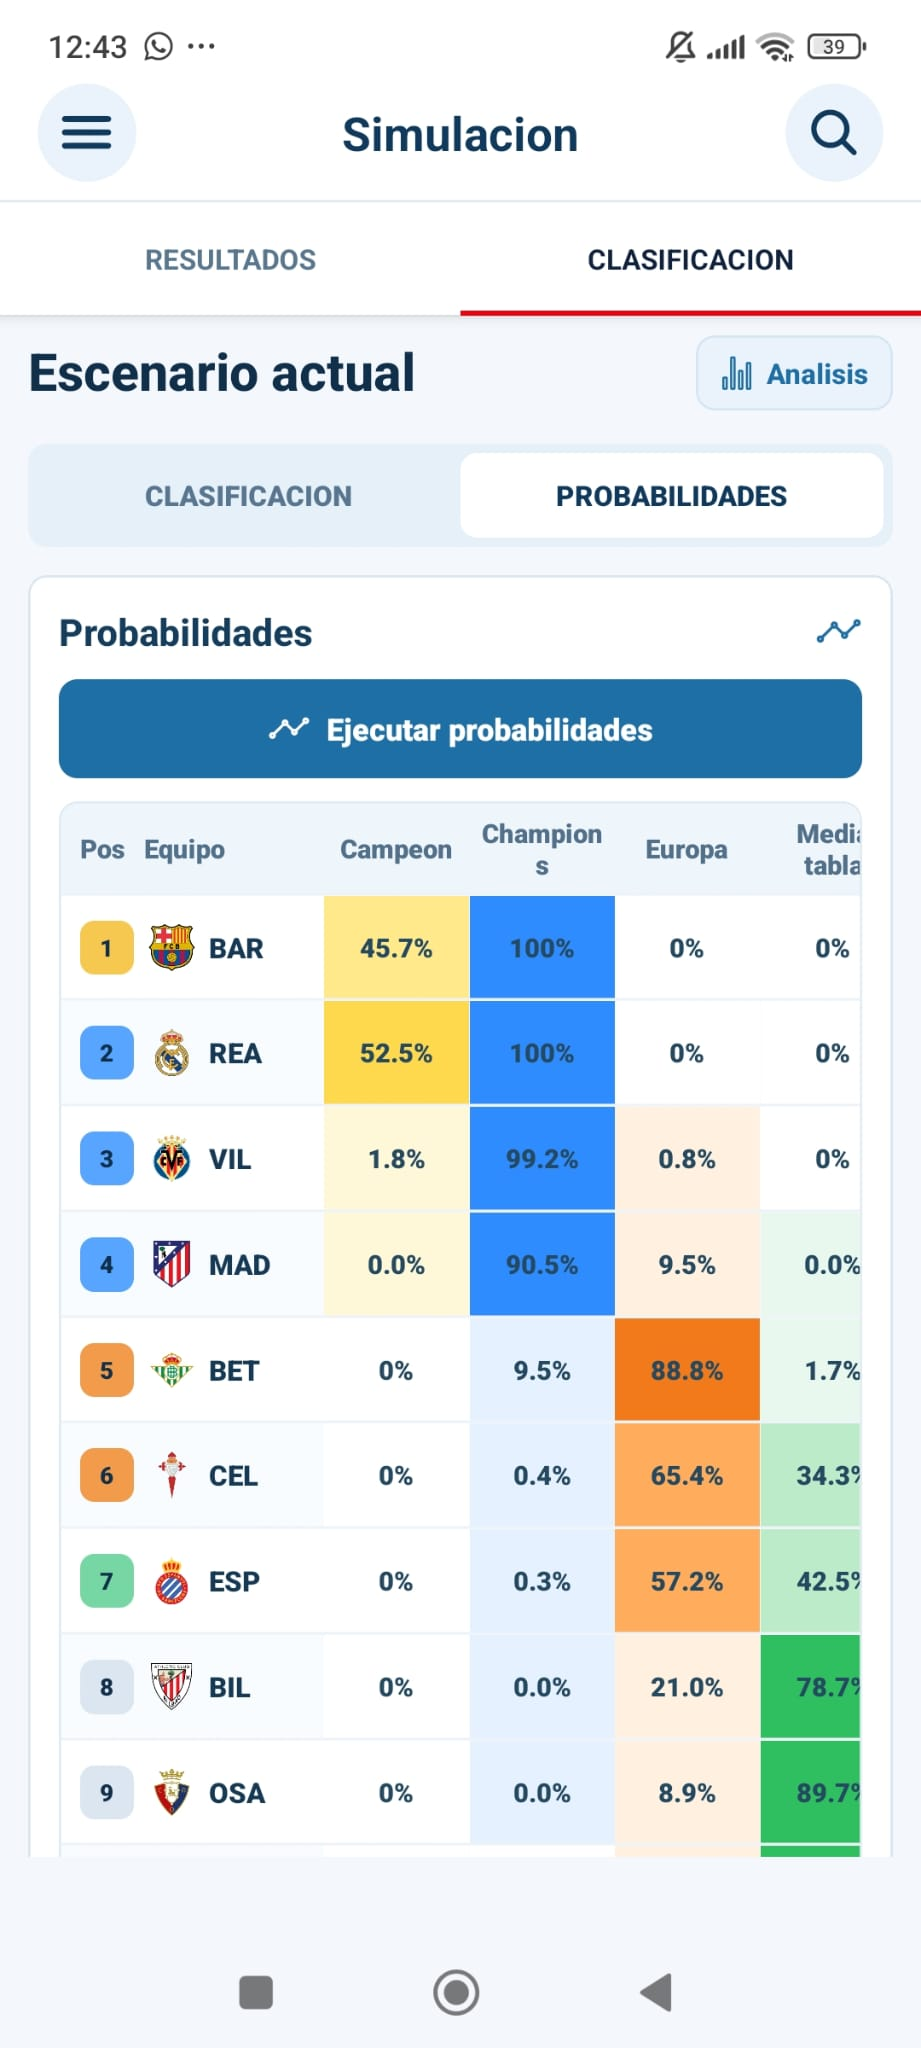
\includegraphics[width=0.8\textwidth]{figures/cap_sim_prob.jpeg}
\caption{Probabilidades}
\label{fig:sim_prob}
\end{subfigure}
\hfill
\begin{subfigure}[b]{0.32\textwidth}
\centering
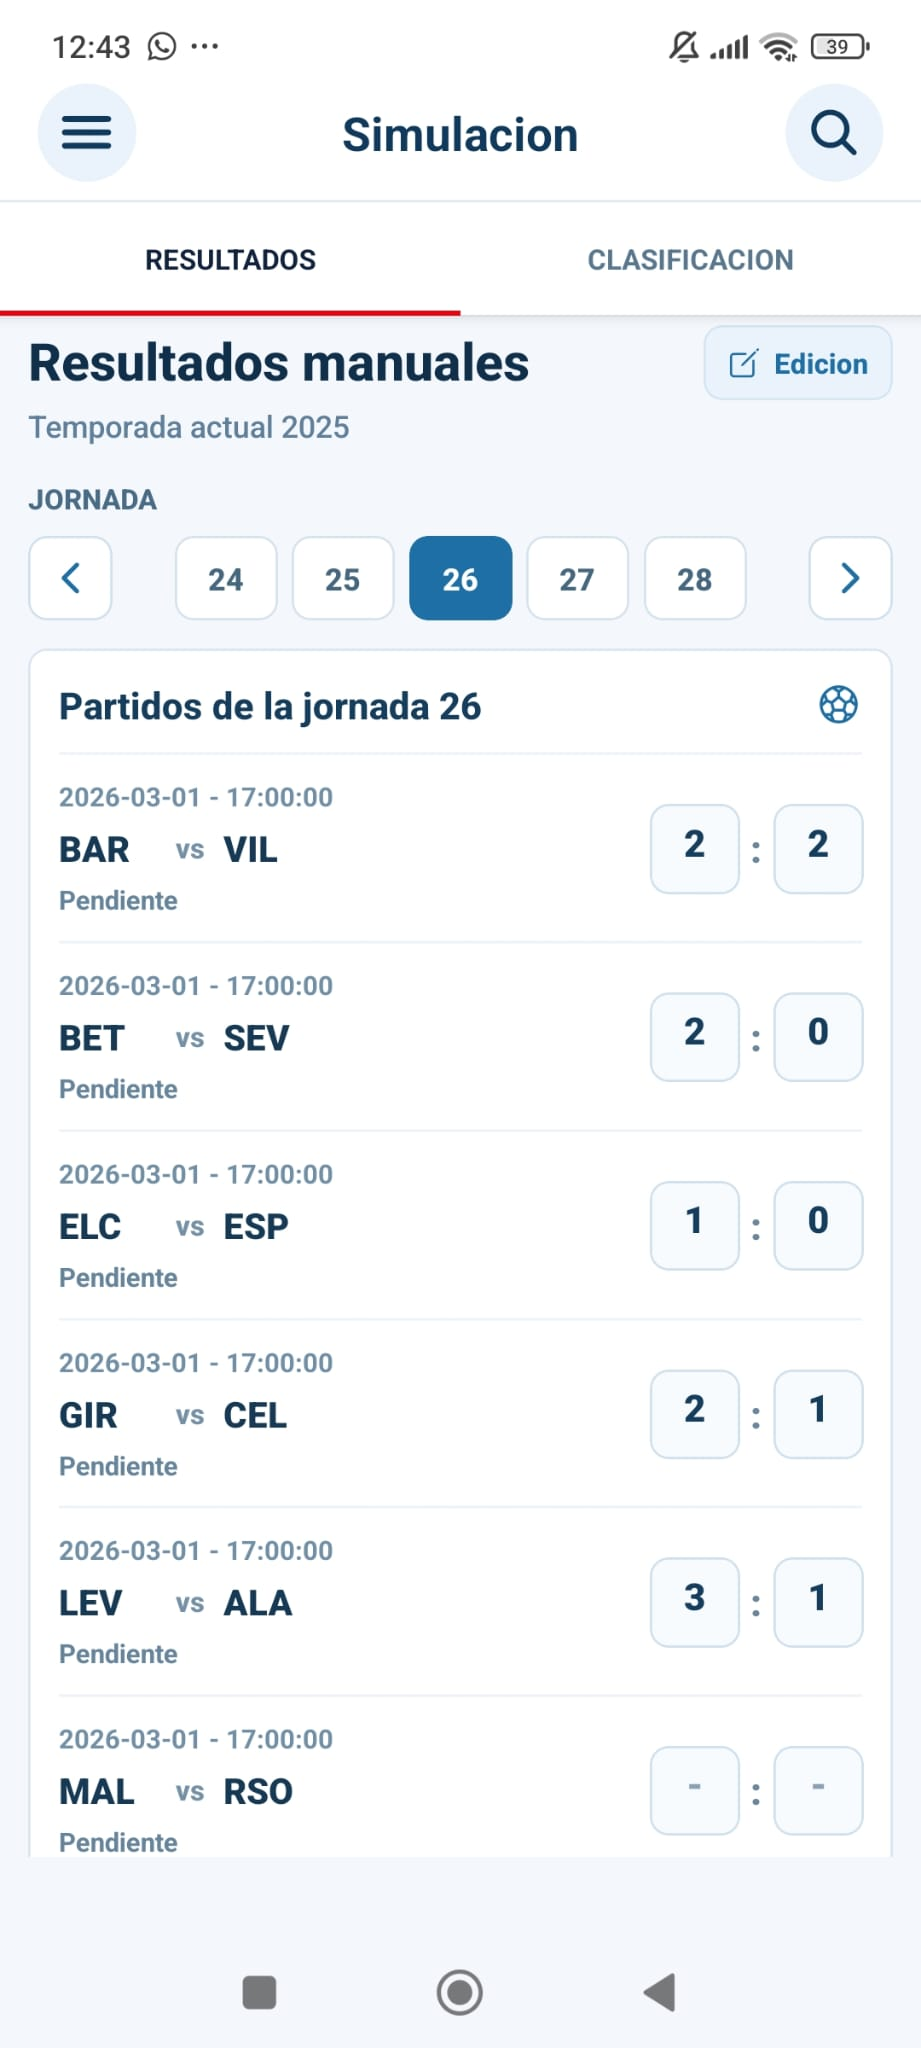
\includegraphics[width=0.8\textwidth]{figures/cap_sim_result.jpeg}
\caption{Resultados}
\label{fig:sim_result}
\end{subfigure}

\caption{Pantallas correspondientes al proceso de simulación}
\label{fig:simulacion}
\end{figure}

Por último, la aplicación incluye diferentes opciones de configuración y personalización de la cuenta, entre ellas la actualización de la contraseña y la adaptación de la interfaz mediante los temas claro y oscuro.

\begin{figure}[H]
\centering
\begin{subfigure}[b]{0.4\textwidth}
\centering
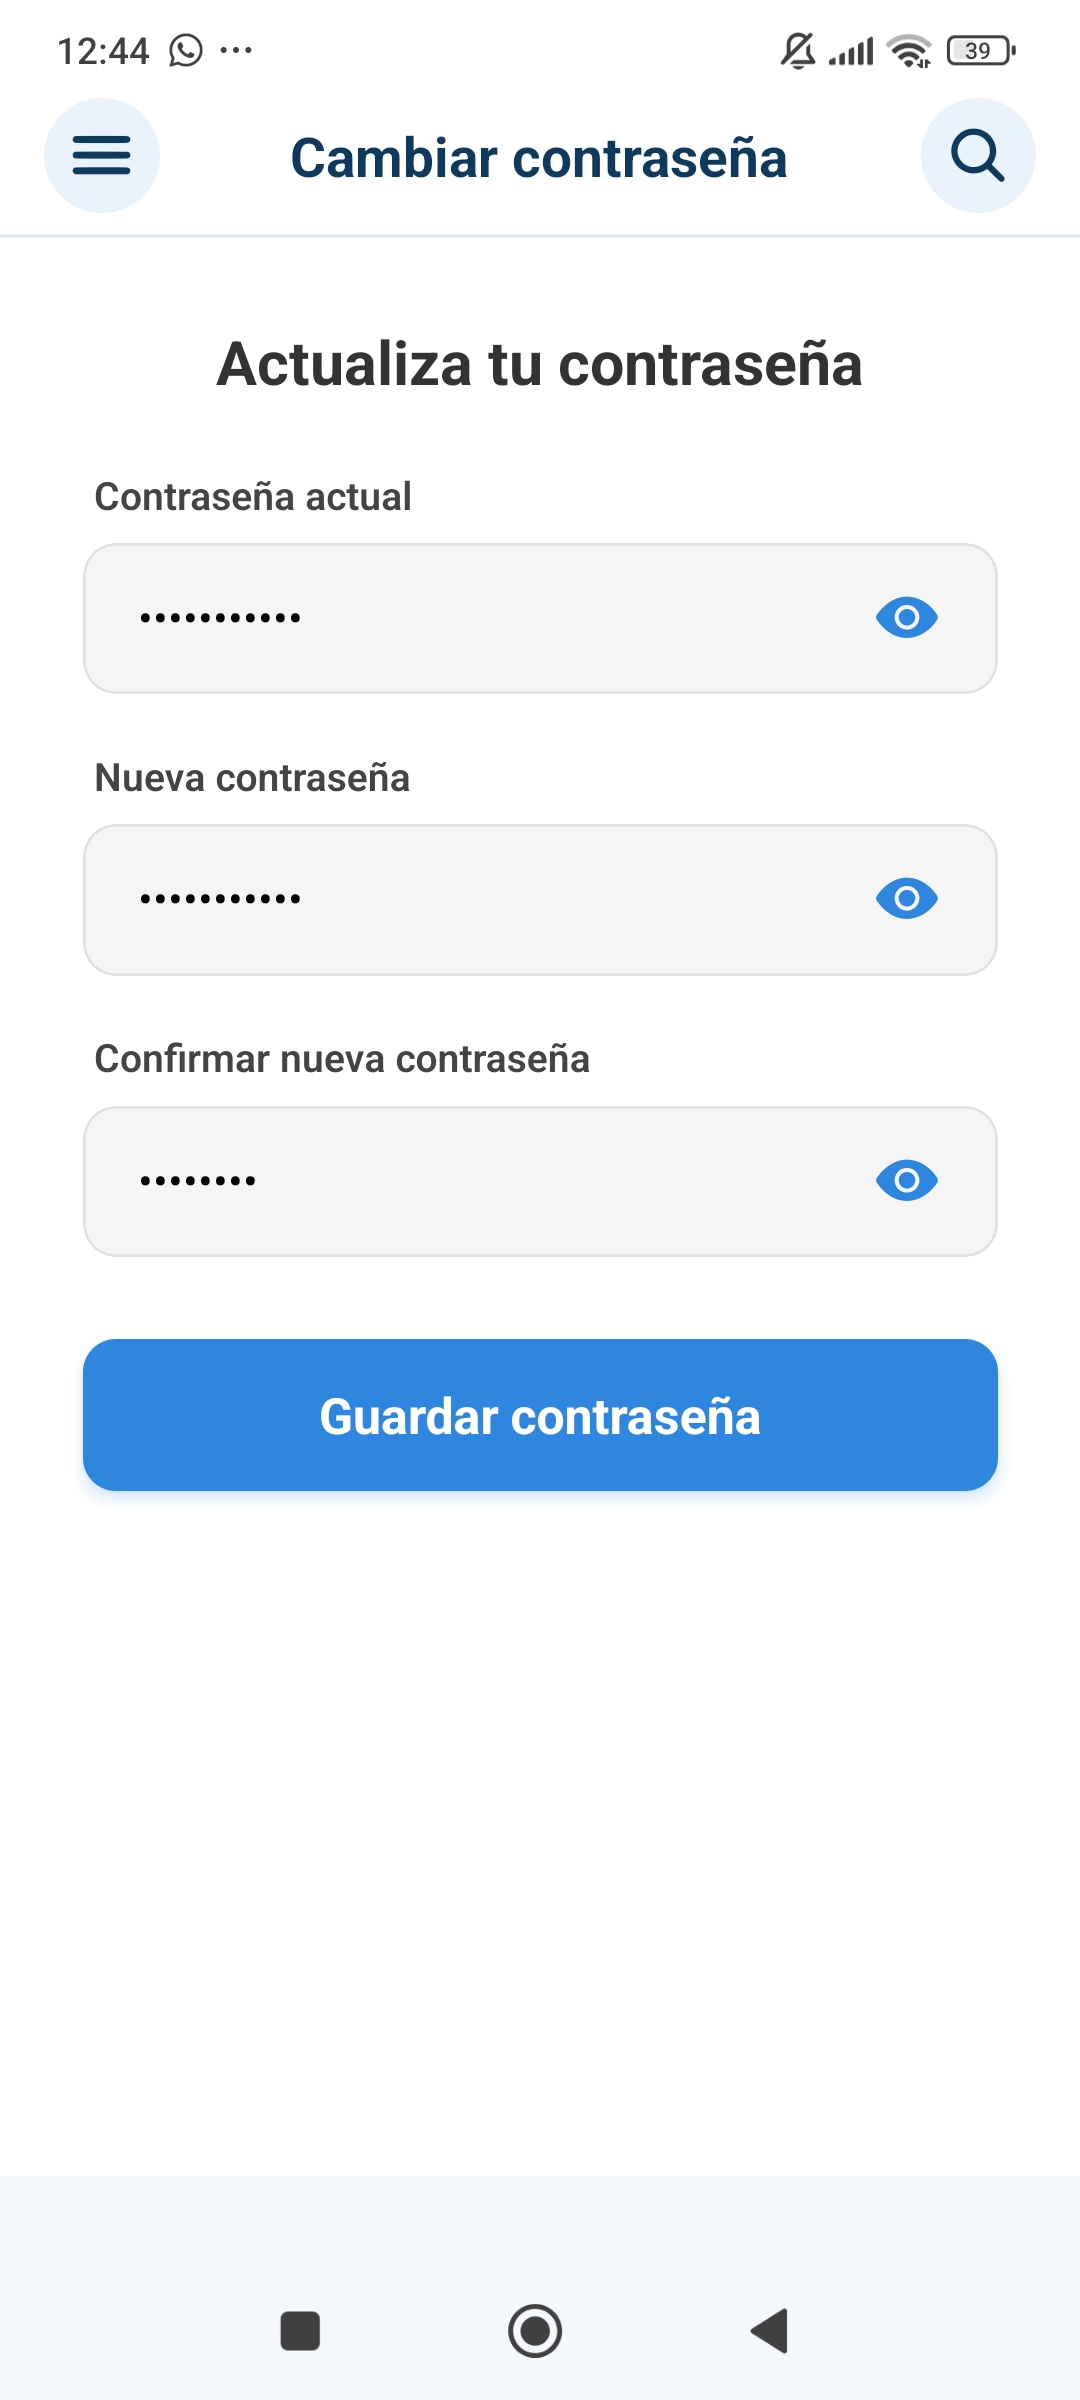
\includegraphics[width=0.5\textwidth]{figures/cap_act_contr.jpeg}
\caption{Actualización de contraseña}
\label{fig:actualizar_contrasena}
\end{subfigure}
\caption{Gestión y configuración de la cuenta}
\label{fig:configuracion}
\end{figure}

\subsection{Logotipo, colores y nombre de la aplicación}

El nombre de la aplicación, \textit{MoneyBall LaLiga}, toma como referencia la película \textit{Moneyball}, basada en la aplicación de métodos estadísticos y analíticos al ámbito deportivo. En dicha obra se muestra cómo el uso de datos puede ayudar a construir un equipo competitivo con recursos económicos limitados, identificando jugadores infravalorados a partir de indicadores objetivos de rendimiento. Esta idea se relaciona directamente con la finalidad del presente Trabajo Fin de Grado, ya que la aplicación busca facilitar el análisis de datos futbolísticos y apoyar la interpretación del rendimiento de equipos y jugadores. Además, se incorpora el término \textit{LaLiga} debido a que el proyecto se centra exclusivamente en esta competición.

En cuanto al logotipo, mostrado en la Figura~\ref{fig:logo}, se diseñó con apoyo de una herramienta de generación de imágenes basada en inteligencia artificial. Para su creación se partió de la idea de una aplicación denominada \textit{MoneyBall LaLiga}, utilizando tonos azules y una representación sencilla de elementos relacionados con gráficos y análisis de datos. El objetivo era obtener una imagen visual sobria, minimalista y coherente con el carácter analítico de la aplicación, evitando un diseño excesivamente recargado.

\begin{figure}[H]
    \centering
    
\includegraphics[width=0.6\linewidth]{figures/logo.png}
    \caption{Logo de la app.}
    \label{fig:logo}
\end{figure}

A partir de esta identidad visual se seleccionó una paleta principal basada en tonos azules. Esta elección busca transmitir una imagen tecnológica, limpia y profesional, manteniendo al mismo tiempo un contraste adecuado para los distintos elementos de la interfaz. La paleta fue elaborada mediante la herramienta Coolors y se muestra en la Figura~\ref{fig:paleta}.

\begin{figure}[H]
    \centering
    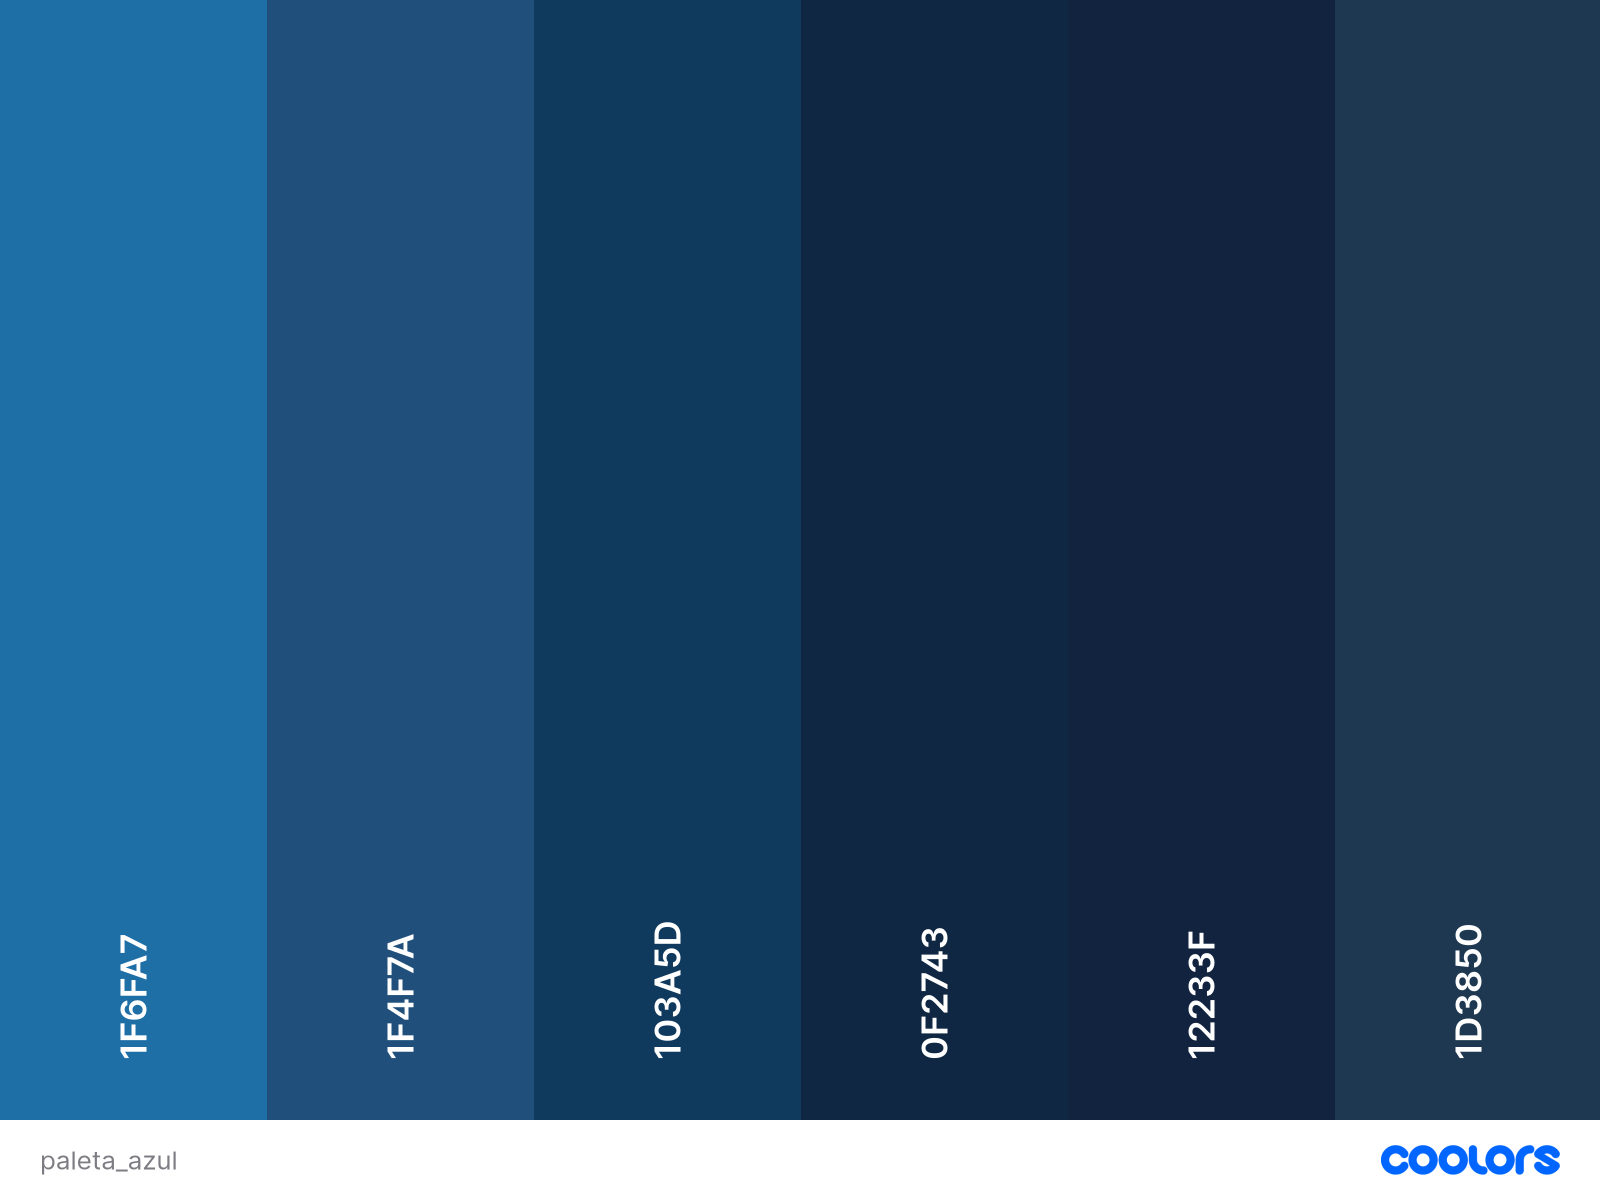
\includegraphics[width=0.8\linewidth]{figures/paleta_azul.png}
    \caption{Paleta de colores.}
    \label{fig:paleta}
\end{figure}

Para los fondos de la aplicación se escogió una combinación de colores claros y suaves, con el objetivo de favorecer la legibilidad y resaltar el azul principal utilizado en botones, encabezados y elementos interactivos. Esta paleta complementaria puede observarse en la Figura~\ref{fig:paleta_fondo}.

\begin{figure}[H]
    \centering
    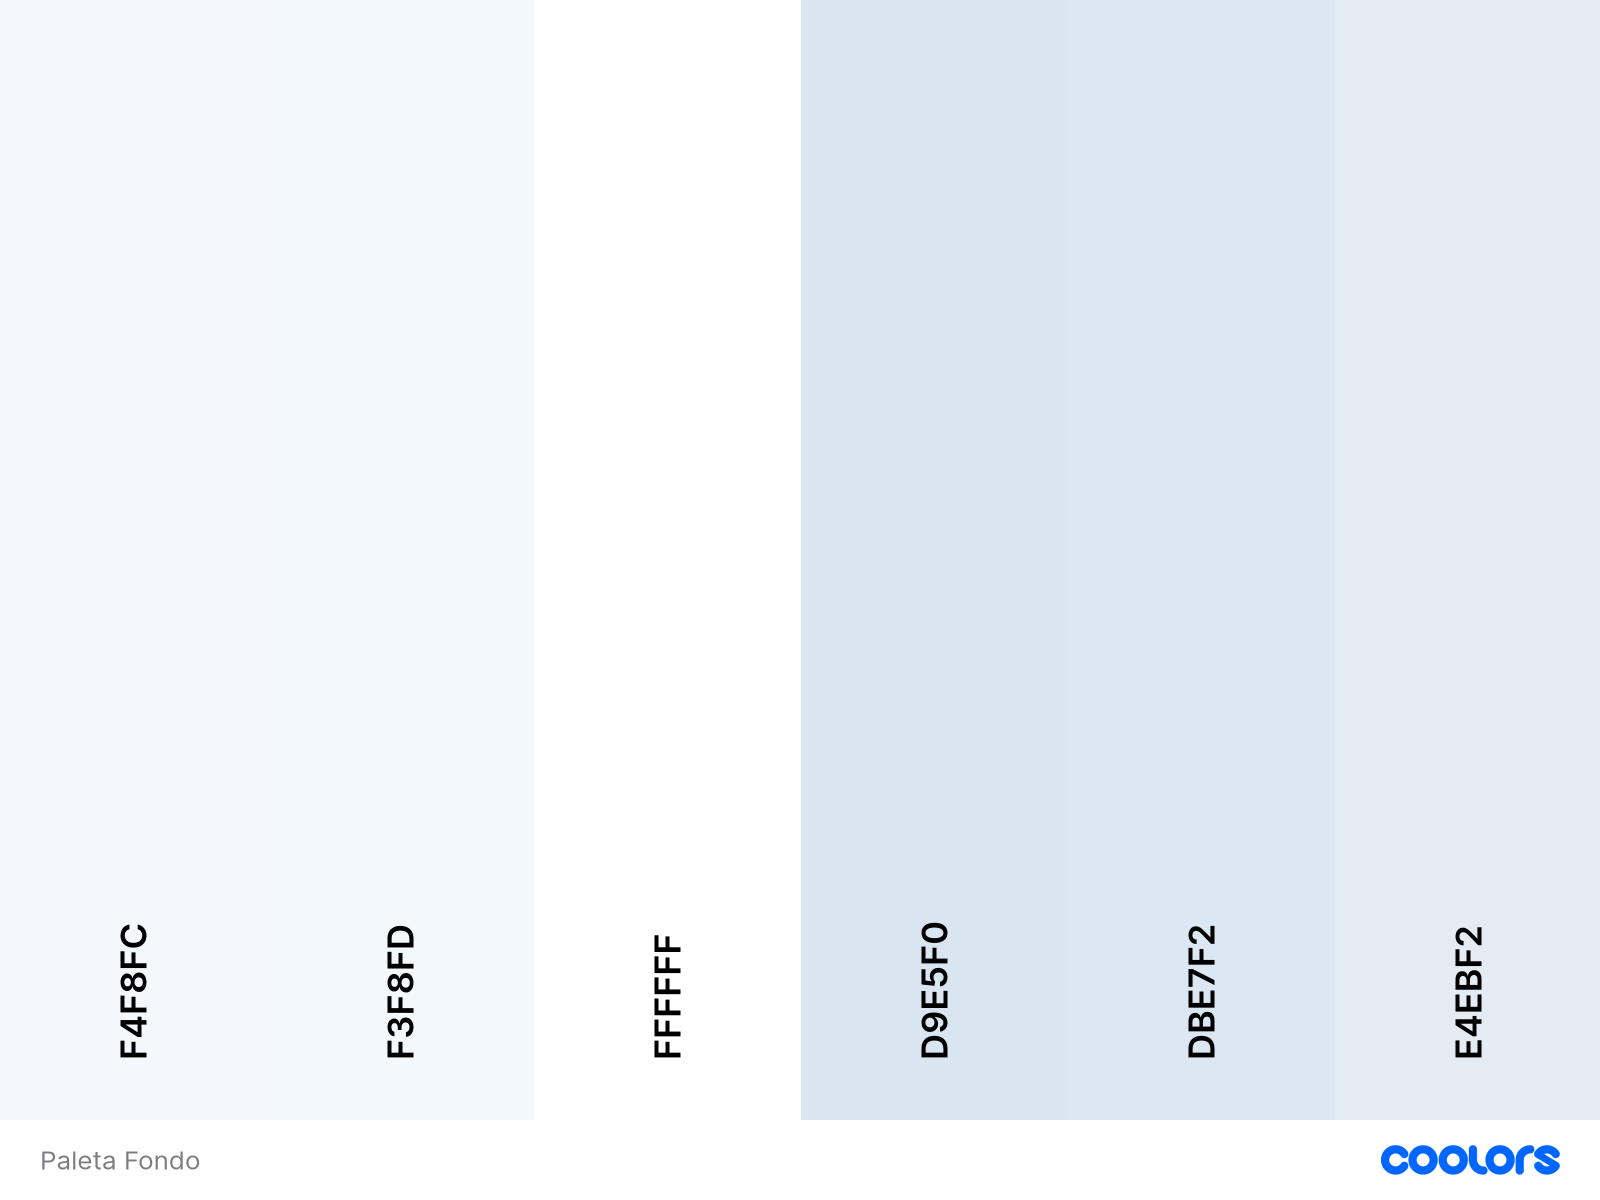
\includegraphics[width=0.8\linewidth]{figures/Paleta Fondo.png}
    \caption{Paleta de fondos.}
    \label{fig:paleta_fondo}
\end{figure}

Además, se definió una paleta específica para la pantalla del asistente conversacional, denominado \textit{Agente de oro}. En este caso se emplean tonos dorados con distintos niveles de contraste, con el fin de diferenciar visualmente esta funcionalidad del resto de la aplicación y reforzar su identidad propia dentro del sistema. La paleta correspondiente se recoge en la Figura~\ref{fig:paleta_agente}.

\begin{figure}[H]
    \centering
    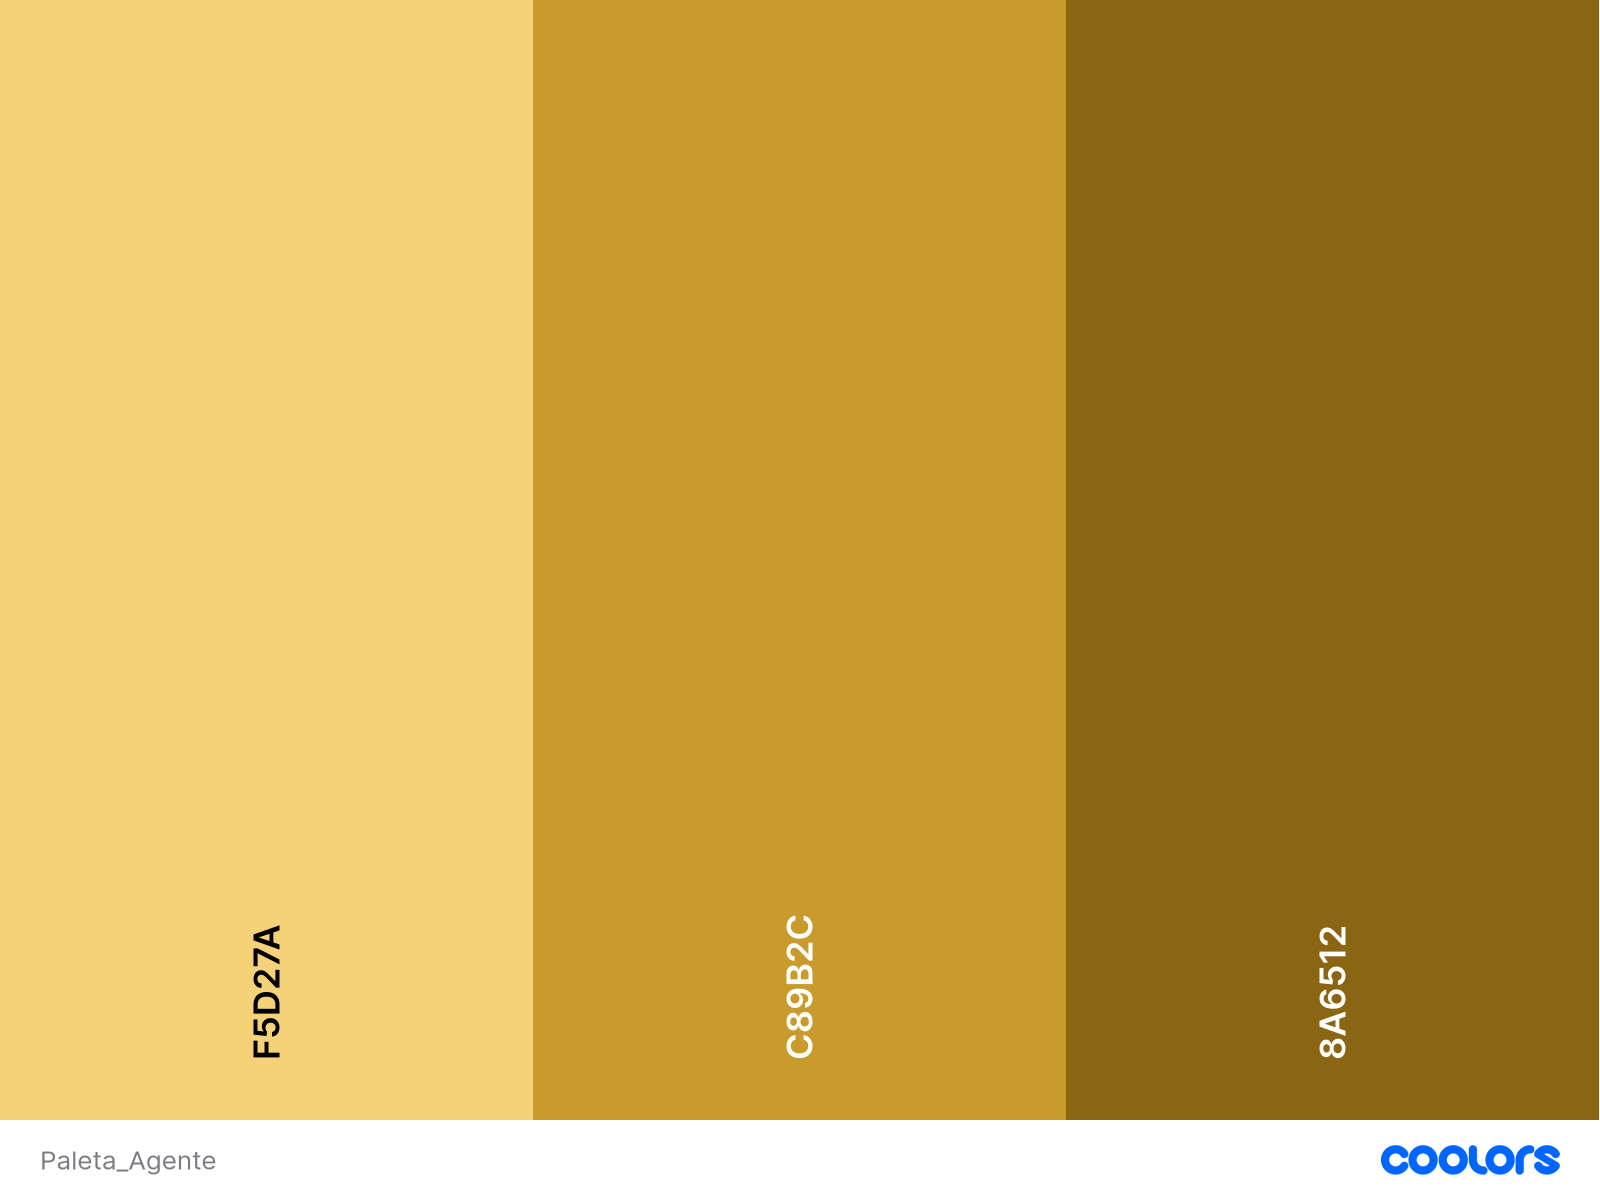
\includegraphics[width=0.8\linewidth]{figures/Paleta_Agente.png}
    \caption{Paleta de Agente de oro.}
    \label{fig:paleta_agente}
\end{figure}

Por último, para el modo oscuro se mantiene la misma línea visual basada en tonos azules, pero adaptada a fondos más oscuros. En este caso, los fondos de las pantallas y tarjetas emplean colores oscuros, mientras que los textos y elementos principales utilizan tonos claros para asegurar una correcta legibilidad. De esta forma, el modo oscuro conserva la identidad visual de la aplicación y ofrece una alternativa más cómoda en entornos con poca iluminación.